\documentclass{article}
\usepackage[utf8]{inputenc}
\usepackage[T1]{fontenc}
\usepackage{microtype}
\usepackage{graphicx}
%\usepackage{hyperref}
\usepackage{amsmath}
\usepackage{booktabs}
\usepackage{longtable}
\usepackage{array}
\usepackage{multirow}
\usepackage{caption}
\usepackage{subcaption}
\usepackage{geometry}
\usepackage{xcolor}
\usepackage{listings}
\usepackage{float}
\usepackage{tabularx}
\geometry{margin=1in}
\usepackage{listings}

%\usepackage{biblatex}
\usepackage[backend=biber,style=ieee]{biblatex}
\addbibresource{references.bib}  
\usepackage{longtable}

\usepackage[acronym]{glossaries}
\makeglossaries

\newacronym{sar}{SAR}{Synthetic Aperture Radar}
\newacronym{map}{mAP}{Mean Average Precision}
\newacronym{smart}{SMART}{Specific, Measurable, Achievable, Relevant, Time-bound}
\newacronym{ais}{AIS}{Automatic Identification System}
\newacronym{yolov8}{YOLOv8}{You Only Look Once version 8 (a machine learning model for object detection)}
\newacronym{deepsort}{DeepSort}{Simple Online and Realtime Tracking with a Deep Association Metric}
\newacronym{yolov11m}{YOLOv11m}{You Only Look Once version 11 medium (a machine learning model for object detection)}
\newacronym{coco}{COCO dataset}{Common Objects in Context dataset}
\newacronym{onnx}{ONNX}{Open Neural Network Exchange}
\newacronym{tensorrt}{TensorRT}{NVIDIA TensorRT (an SDK for high-performance deep learning inference)}
\newacronym{sdk}{SDK}{Software Development Kit}
\newacronym{grd}{GRD}{Ground Range Detected (a type of SAR product)}
\newacronym{far}{FAR}{False Alarm Rate}
\newacronym{ssdd}{SSDD}{SAR Ship Detection Dataset}
\newacronym{dssdd}{DSSDD}{Dual-Polarimetric SAR Ship Detection Dataset}
\newacronym{hrsid}{HRSID}{High-Resolution SAR Images Dataset}
\newacronym{ivision}{iVision-MRSSD}{A multi-resolution SAR ship detection dataset for satellite based maritime surveillance applications}
\newacronym{ssd}{SSD}{Single Shot MultiBox Detector}
\newacronym{cfar}{CFAR}{Constant False Alarm Rate}
\newacronym{cnn}{CNN}{Convolutional Neural Network}
\newacronym{dcenn}{DCENN}{Dense Connected Neural Network}
\newacronym{phbt}{PHBT}{Pure Background Hybrid Training}
\newacronym{cta}{CTA}{Computed Tomography Angiography (Similar technique used for SAR data)}
\newacronym{memae}{MemAE}{Memory-Augmented Autoencoder}
\newacronym{vv}{VV polarization}{Vertical transmit, Vertical receive polarization}
\newacronym{vh}{VH polarization}{Vertical transmit, Horizontal receive polarization}
\newacronym{hh}{HH polarization}{Horizontal transmit, Horizontal receive polarization}
\newacronym{snap}{SNAP}{Sentinel Application Platform (software for SAR data processing)}
\newacronym{api}{API}{Application Programming Interface}
\newacronym{rcs}{RCS}{Radar Cross-Section}
\newacronym{scr}{SCR}{Signal-to-Clutter Ratio}
\newacronym{lts}{LTS}{Long Term Support}
\newacronym{cuda}{CUDA}{Compute Unified Device Architecture}
\newacronym{cudnn}{cuDNN}{CUDA Deep Neural Network library}
\newacronym{lpddr4}{LPDDR4}{Low Power Double Data Rate 4}
\newacronym{mota}{MOTA}{Multiple Object Tracking Accuracy}
\newacronym{hota}{HOTA}{Higher Order Tracking Accuracy}
\newacronym{scp}{SCP}{Secure Copy Protocol}
\newacronym{fp16}{FP16}{Half-precision floating-point format}
\newacronym{cv2}{CV2}{Open Source Computer Vision Library}
\newacronym{numpy}{Numpy}{Numerical Python}
\newacronym{ort}{ort}{ONNX Runtime}
\newacronym{pytorch}{PyTorch}{An open-source machine learning framework}
\newacronym{yaml}{YAML}{YAML Ain't Markup Language}
\newacronym{tpu}{TPU}{Tensor Processing Unit}
\newacronym{asic}{ASIC}{Application-Specific Integrated Circuit}
\newacronym{relu}{ReLU}{Rectified Linear Unit}


\usepackage[colorlinks=true, linkcolor=black, urlcolor=black, citecolor=black]{hyperref}

\hyphenpenalty 10000







\lstset{
  language=Python,
  backgroundcolor=\color{gray!10},
  basicstyle=\ttfamily\small,
  keywordstyle=\color{blue},
  stringstyle=\color{red},
  commentstyle=\color{gray},
  showstringspaces=false,
  frame=single,
  breaklines=true,
}



\geometry{a4paper, margin=1in}

\title{\acrshort{sar} Ship Detection Project Documentation}
\author{Chahine, Yan, Nadezhda, Anna, Stevie}
\date{July 24, 2025}

\begin{document}
\sloppy

\maketitle

\begin{abstract}
This document outlines the \acrshort{sar} Ship Detection Project, aiming to detect and track ships using Synthetic Aperture Radar (\acrshort{sar}) data from sources like Sentinel-1. The core functionality involves machine learning models for land-sea segmentation and image correction, together with deep learning models for ship detection and tracking. The system offers three user interfaces: a Jetson Nano for on-orbit inference and data downlink, a web-based interface for on-demand analysis of \acrshort{sar} data selected via a \acrshort{map}, and an image upload feature for user-provided raw \acrshort{sar} imagery. Key objectives include developing lightweight, high-accuracy models for real-time ship identification, tracking, and potential applications such as monitoring illegal activities, aiding in search and rescue operations, and general maritime surveillance. \\\\Associated Code Repository: https://github.com/ioEclipse/\acrshort{sar}-SHIP-DETECTION 


\end{abstract}
\newpage
\tableofcontents
\newpage
\section{Introduction}
%%This section provides an overview of the \acrshort{sar} Ship Detection project, its objectives, and its significance.
\subsection{Project Overview}Initiated as an intensive, one-month endeavor, the \acrshort{sar} Ship Detection Project is engineered to establish a comprehensive and highly functional system for the detection and persistent tracking of maritime vessels from Synthetic Aperture Radar (\acrshort{sar}) imagery. The project's technical backbone is built around ingesting and intelligently processing \acrshort{sar} data, with a primary focus on data derived from the Sentinel-1 satellite constellation, though the architecture supports extensibility to other \acrshort{sar} sources.\\

Our workflow is meticulously designed: raw \acrshort{sar} images undergo a series of crucial preprocessing steps, including algorithms for accurate land-sea demarcation and the mitigation of inherent speckle noise, ensuring optimal feature extraction. The clean data is then fed into a machine learning pipeline featuring \acrshort{yolov11m} for robust ship object detection. \\

A key innovation of this project lies in its three-tiered accessibility model: a compact, high-performance solution designed for deployment on edge devices such as the NVIDIA Jetson Nano, reflecting our foresight into future space-based or remote applications; an intuitive web application allowing users to specify areas of interest on a map for near real-time \acrshort{sar} analysis; and a direct image upload feature for immediate processing of user-provided raw \acrshort{sar} files. This project seeks to provide a versatile toolset for applications ranging from enhanced maritime surveillance and environmental monitoring to critical support for search and rescue missions.\\

The \acrshort{sar} Ship Detection Project aims to address the critical need for robust and automated solutions in maritime surveillance. Traditional methods for ship detection often rely on visual inspections, which are labor-intensive, time-consuming, and limited by environmental factors like darkness or adverse weather conditions. Synthetic Aperture Radar (\acrshort{sar}) offers an all-weather, day-and-night imaging capability, making it highly suitable for continuous maritime monitoring.\\

However, extracting reliable ship information from \acrshort{sar} imagery presents several significant challenges:
\begin{itemize}
    \item \textbf{Speckle Noise}: \acrshort{sar} images are inherently affected by speckle noise, a granular appearance that can obscure targets and make accurate ship detection difficult, especially for smaller vessels. \item \textbf{Varying Ship Sizes and Orientations}: Ships can vary significantly in size, shape, and orientation, leading to diverse radar signatures. A robust detection system must be able to identify these variations effectively. \item \textbf{Cluttered Environments}: Coastal areas and busy shipping lanes often present cluttered environments, where ships may be difficult to distinguish from landmasses, offshore structures, or other marine clutter. \item \textbf{Need for Automated Monitoring}: The vastness of oceanic environments necessitates automated monitoring solutions to efficiently track ship movements, identify anomalies, and support applications such as maritime safety, illegal fishing prevention, and border security. \item \textbf{Data Volume and Processing}: The increasing availability of high-resolution \acrshort{sar} data, such as from Sentinel-1, generates massive volumes of information that require efficient and automated processing techniques to extract actionable intelligence. \end{itemize}

This project seeks to overcome these challenges by developing machine learning algorithms capable of accurately identifying and tracking ships within \acrshort{sar} imagery, thereby enabling effective and automated maritime surveillance. \subsection{Problem Statement}
The escalating crisis of irregular immigration across the Mediterranean Sea, intertwined with the socioeconomic devastation from illegal fishing in West African waters and the escalating geopolitical tensions exemplified by the Russia-Ukraine conflict, has precipitated a dire need for enhanced maritime domain awareness. This region has witnessed over 3,000 migrant deaths in 2023 alone, with a cumulative toll exceeding 20,000 since 2014 due to perilous crossings, while illegal fishing has reduced Senegal’s catches by 37\% between 2000 and 2016, displacing fishers and fueling migration. \\

Synthetic aperture radar (\acrshort{sar}) data, with its all-weather and day-night imaging capabilities, offers a critical resource for ship detection and tracking; however, its effective utilization hinges on advanced artificial intelligence (AI) integrated with edge computing, particularly on CubeSats, to enable real-time analysis, reduce data transmission burdens, and deliver precise insights. \\

Existing algorithms in the literature consistently fall short in achieving the requisite precision, response time, generalizability, and successful implementation and testing in real-world scenarios. To address these gaps, the following questions are posed:
\begin{itemize}
    \item How can AI at the edge of CubeSats reduce data transmission and enhance real-time decision-making for maritime surveillance? \item How can we design and optimize a high-performance solution for ship detection, tracking, and decision support using \acrshort{sar} data and edge AI technologies? \item How can this solution be implemented and tested in real-world, complex maritime scenarios to ensure reliability and effectiveness? \end{itemize}
\subsection{Project Goals and Objectives}
This project is dedicated to the design, implementation, and deployment of a practical ship‑detection system based on Synthetic Aperture Radar (\acrshort{sar}). By combining state‑of‑the‑art machine learning techniques with real‑world data and edge‑computing platforms, our project delivers a comprehensive end‑to‑end solution tailored for maritime surveillance. \\

To ensure both technical rigor and operational relevance, we have defined the following high‑level goals and \acrshort{smart} objectives:
\begin{itemize}
    \item \textbf{Robust Training Dataset}: Curate and annotate a diverse collection of \acrshort{sar} coverages, including open‑sea, coastal, and congested port scenarios, to achieve at least 10,000 labeled vessel instances by Month 6.
    \item \textbf{Lightweight Inference Models}: Develop and train convolutional neural networks optimized for low‑power inference, targeting an average per‑image inference time under $50\cdot ms$ on desktop GPUs by Month 8.
    \item \textbf{Edge Platform Optimization}: Identify the optimal neural‑network architecture for deployment on the NVIDIA Jetson Nano; implement 8‑bit quantization and \acrshort{tensorrt} acceleration to sustain real‑time processing at $\geq 5\cdot frames$ per second by Month 10.
    \item \textbf{Reliable Object Detection \& Tracking}:Integrate detection and multi‑object tracking modules to maintain persistent vessel identities across at least 95\% of sequential \acrshort{sar} passes in test scenarios by Month 12.
    \item \textbf{\acrshort{ais} Data Fusion}: Correlate \acrshort{sar} detections with \acrshort{ais} broadcasts to confirm $\geq90\%$ of vessel matches, resolve at least 80\% of ambiguous detections, and flag dark‑vessel anomalies for operator review by Month 11.
    \item \textbf{User‑Actionable Outputs}:Generate georeferenced alerts, summary reports, and annotated imagery formatted for rapid ingestion by maritime operators, with average report generation times under $10\cdot seconds$ by Month 12.
    \item \textbf{Multi‑Modal User Interfaces}:Deliver three distinct access modalities: a GPU‑powered web demonstration, an interactive world‑map dashboard, and a local raw‑image upload portal to support diverse end‑user workflows, all operational by thesis defense. \end{itemize}
\subsection{Document Structure}
To ensure comprehensive understanding, this documentation is organized into a logical flow mirroring the project's development lifecycle. \\

It commences with an \textbf{Executive Summary} and \textbf{Introduction }for a concise project overview. The \textbf{Project Context and Justification} grounds the effort in its broader significance, while \textbf{Requirements Specification} meticulously lists all functional and non-functional demands. \\

The core technical details are captured in \textbf{System Design}, explaining both the high-level architecture and individual component designs. \textbf{Implementation and Development} provides the essential "how-to" for reproducing the project's environment and code. \\

The specifics of machine learning are detailed in \textbf{Model Training and Optimization}, leading to the empirical \textbf{Evaluation and Testing} of the system's performance. \\

A practical \textbf{Usage Guide} assists in system operation, and forward-looking sections on \textbf{System Optimization, Known Issues and Troubleshooting}, and \textbf{Future Work} and \textbf{Enhancements} discuss continuous improvement, culminating in the \textbf{Conclusion}. \newpage 

\section{Project Context and Justification}
This section provides background information and the rationale behind the project. \subsection{Motivation}
The \acrshort{sar} Ship Detection Project is motivated by the critical need for enhanced maritime domain awareness and the unparalleled advantages of Synthetic Aperture Radar (\acrshort{sar}) in addressing the limitations of conventional surveillance methods. Oceans serve as the backbone of global trade, security, and ecological balance, necessitating reliable and real-time monitoring of maritime activities. \acrshort{sar} technology, with its all-weather, day-and-night imaging capability, provides a unique solution to this challenge, overcoming the constraints of optical sensors that are hindered by cloud cover, darkness, or adverse weather conditions. The significance of automated \acrshort{sar}-based ship detection spans multiple domains, each with substantial real-world implications:

\begin{itemize}
    \item Maritime Safety \& Security
    \begin{itemize}
        \item Enables search and rescue (\acrshort{sar}) operations by rapidly locating distressed vessels. \item Detects illegal activities, including piracy, smuggling, and unauthorized fishing, ensuring compliance with maritime laws. \item Enhances border security by monitoring territorial waters and identifying suspicious vessel movements. \end{itemize}
    \item Defense \& National Security
    \begin{itemize}
        \item Supports naval surveillance by tracking warships, submarines, and other strategic assets. \item Provides intelligence-gathering capabilities in contested or remote maritime regions. \item Improves situational awareness in critical waterways (e.g., straits, exclusive economic zones). \end{itemize}
    \item Economic \& Commercial Applications
    \begin{itemize}
        \item Optimizes shipping logistics by analyzing vessel traffic patterns and route efficiency. \item Aids port management and maritime insurance through real-time vessel tracking. \item Facilitates trade monitoring by verifying cargo movements and detecting anomalies. \end{itemize}
    \item Environmental \& Resource Protection
    \begin{itemize}
        \item Prevents illegal, unreported, and unregulated (IUU) fishing in protected marine zones. \item Monitors offshore infrastructure (e.g., oil rigs, wind farms) for security and maintenance. \item Supports disaster response by assessing ship movements during oil spills or other marine incidents. \end{itemize}
\end{itemize}
Despite these compelling applications, existing ship detection systems often struggle with speckle noise, cluttered environments, and scalability issues, particularly when processing large volumes of \acrshort{sar} data. This project addresses these gaps by developing a robust, automated, and scalable detection framework that leverages deep learning (YOLOv11) to deliver actionable maritime intelligence. By harnessing \acrshort{sar}’s unique capabilities, this work aims to bridge the divide between data availability and operational decision-making, ultimately contributing to safer, more secure, and sustainably managed oceans. \subsection{Literature Review and Background}
Synthetic Aperture Radar (\acrshort{sar}) ship detection is a cornerstone of maritime surveillance, leveraging its all-weather, day-and-night imaging capabilities to monitor vessels across diverse conditions. Traditional methods, such as Constant False Alarm Rate (CFAR) detectors, have been foundational but often suffer from high false alarm rates in complex backgrounds and struggle to detect small or closely spaced ships. These limitations have driven the adoption of deep learning techniques, which offer superior feature extraction and pattern recognition. Since 2017, significant advancements have been made through innovative algorithms and specialized datasets, addressing challenges like multiscale imbalances, variable ship sizes, and complex environments. \\

In 2017, \cite{8124934} introduced an improved Faster R-\acrshort{cnn} model tailored for \acrshort{sar} ship detection, utilizing the \acrshort{sar} Ship Detection Dataset (SSDD) with 1,160 images (500×500 pixels, 1–15 m resolution) from Sentinel-1, RadarSat-2, and TerraSAR-X. By incorporating feature fusion, transfer learning, and hard negative mining, their approach achieved higher accuracy and lower computational cost than traditional methods, setting a precedent for deep learning in this domain. Concurrently, \cite{8067489} developed OpenSARShip 2.0, a dataset with 34,528 Sentinel-1 ship chips (30×30 to 120×120 pixels, 2 m resolution), integrated with \acrshort{ais} information and enhanced with interference labeling and type classification, enabling deeper ship target interpretation.\\

In 2018, \cite{8124929} introduced the OpenSARShip dataset, comprising 11,346 Sentinel-1 ship chips (30×30 to 120×120 pixels, 2.2 m resolution), designed as a benchmark for ship interpretation algorithms due to its large scale, diversity, and reliability. Building on this, \cite{rs11070765} constructed a \acrshort{sar} dataset with 39,729 ship chips (256×256 pixels, 3–25 m resolution) from 102 Gaofen-3 and 108 Sentinel-1 images, supporting robust object detection in complex backgrounds without land-ocean segmentation. \\

Similarly, \cite{R19097} released AIR-SARShip-1.0, with 31 Gaofen-3 images (500×500 pixels, 1–3 m resolution), achieving an average precision of 88.1\% using density-connected neural networks, addressing data scarcity in high-resolution \acrshort{sar} imagery. \\

In 2020, \cite{rs12182997}. presented LS-\acrshort{ssdd}-v1.0, a dataset of 9,000 Sentinel-1 sub-images (800×800 pixels) focused on small ship detection, introducing a Pure Background Hybrid Training mechanism to suppress false alarms, validated through ablation studies. \\

In 2021, \cite{rs13245104} released SRSDD-v1.0, containing 666 Gaofen-3 images (1024×1024 pixels, 1 m resolution) with 2,844 ships across six categories, tackling rotated frame detection in nearshore environments. Also in 2021, \cite{s21248478} introduced the Dual-Polarimetric \acrshort{sar} Ship Detection Dataset (\acrshort{dssdd}), with 1,236 Sentinel-1 image slices (256×256 pixels, 3,540 ships), proposing a Memory-Augmented Autoencoder that achieved a mean average precision (\acrshort{map}) of 0.94 by leveraging \acrshort{vv} and VH polarization data to reduce false alarms. \\

Advancing to 2024, \cite{tan2024yolo} proposed YOLO-RC for range-compressed domain detection, achieving an F-score of 88.84\% and average precision of 84.09\% on a self-built dataset, enhancing real-time capabilities by exploiting amplitude gradients and geometric loss. \\

Finally, \cite{sun2025arbitrary} developed an enhanced YOLO network with Shuffle Re-parameterization, Space-to-Depth, and Hybrid Attention modules, achieving AP50 scores of 77.2\%, 91\%, and 95\% on LS-\acrshort{ssdd}, \acrshort{hrsid}, and Vision-MRSSD datasets, respectively, significantly improving small ship detection. \\

Despite these advancements, critical gaps remain, including the limited inclusion of \acrshort{vv} and \acrshort{vh} polarization data in datasets like \acrshort{ssdd} and OpenSARShip, which hinders differentiation of ships from background clutter. Additionally, the restricted resolution range in many datasets limits model generalization across operational conditions, and challenges persist in detecting small ships in complex nearshore environments. \\

Future research should prioritize diverse datasets with multi-polarization data, broader resolution ranges, and advanced feature extraction techniques to enhance detection accuracy and robustness, paving the way for more reliable \acrshort{sar} ship detection systems.\\


These details are organized in Table~\ref{tab:sar_ship_detection} to provide a clearer comparison. \begin{table}%[h!]
\centering
\footnotesize
\begin{tabularx}{\textwidth}{@{}lXlXl@{}}
\toprule
\textbf{Author \& Year} & \textbf{Method} & \textbf{No. of Images \& Shapes} & \textbf{Sensors} & \textbf{Resolution} \\
\midrule
Li et al. (2017) \cite{8124934} & Improved Faster R-\acrshort{cnn} & 1,160 (500 × 500) & Sentinel-1 & 1–15 m \\
Huang et al. (2018) \cite{8124929} & \acrshort{yolov8} & 11,346 (30 × 30 to 120 × 120) & Sentinel-1, Gaofen-3 & 2–22 m \\
Wang et al. (2019) \cite{rs11070765} & Modified \acrshort{ssd} & 43,819 (256 × 256) & Gaofen-3, Sentinel-1 & 3–25 m \\
Sun et al. (2019) \cite{R19097} & Dense connected network (\acrshort{dcenn}) & 1,116 (500 × 500) & Gaofen-3 & 1–3 m \\
Wei et al. (2020) \cite{9127939} & \acrshort{cnn}-based detection/segmentation & 5,604 (800 × 800) &   & 0.5–3 m \\
Zhang et al. (2020) \cite{rs12182997} & Pure Background Hybrid Training (\acrshort{phbt}) & 9,000 (800 × 800) & Sentinel-1 & 10 m \\
Lei et al. (2021) \cite{rs13245104} & Rotated detectors, \acrshort{cta}-based & 666 (1024 × 1024) & Gaofen-3 & 1 m \\
Hu et al. (2021)  \cite{s21248478} & R3Det and YOLOv4 with \acrshort{memae} & 1,236 (256 × 256) & Sentinel-1 & 10 m \\
Tan et al. (2024) \cite{tan2024yolo} & YOLO-RC & \acrshort{hrsid} and \acrshort{ssdd} & Sentinel-1, TerraSAR-X, TanDEM-X & 0.5–15 m \\
Tang et al. (2024) \cite{tang2024dbw} & DBW-YOLO (YOLOv7-tiny) & 5,604 (\acrshort{hrsid}), 1,160 (\acrshort{ssdd}) & Sentinel-1, TerraSAR-X, TanDEM-X & 0.5–15 m \\
Sun et al. (2025) \cite{sun2025arbitrary} & MSDFF-Net & R-\acrshort{ssdd}, R-\acrshort{hrsid} & Sentinel-1, TerraSAR-X, TanDEM-X & 0.5–15 m \\
Guan et al. (2025) \cite{guan2025sar} & Enhanced YOLO (SR module) & \acrshort{hrsid} and \acrshort{ivision}-MRSSD & Sentinel-1, TerraSAR-X, TanDEM-X & 0.5–15 m \\
\bottomrule
\end{tabularx}
\caption{Summary of Public Datasets and Deep Learning Methods for \acrshort{sar} Ship Detection}
\label{tab:sar_ship_detection}
\end{table}

\subsection{ Mission Success Criteria}
The success of the \acrshort{sar} Ship Detection Project will be evaluated based on a combination of technical performance metrics and operational capabilities. The following specific and verifiable criteria must be met:
\begin{enumerate}
    \item Detection Accuracy (Recall \& Precision):
    \begin{enumerate}
        \item The system shall achieve a detection recall of at least $85\%$ for vessels greater than 10 meters in length on a diverse, unseen Sentinel-1 test dataset (e.g., GRD data covering various oceanic environments). \item The system shall achieve a detection precision of at least 90\% for vessels greater than 10 meters in length on the same test dataset. \item The false alarm rate (\acrshort{far}) for land-based clutter and other non-ship targets shall be kept below 0.1\% for open ocean scenes. \end{enumerate}

    \item Processing Speed:
    \begin{enumerate}
        \item The system shall process a standard Sentinel-1 \acrshort{grd} \acrshort{sar} image tile (approximately 25 km x 25 km, depending on resolution) within 30 seconds on the target processing hardware (e.g., a modern GPU-equipped workstation). \item The system shall demonstrate the ability to process consecutive \acrshort{sar} images for tracking purposes with a latency not exceeding 5 seconds per image after initial detection. \end{enumerate}

    \item Tracking Performance:
    \begin{enumerate}
        \item The integrated tracking algorithms shall successfully associate at least 95\% of consecutive ship detections belonging to the same vessel over a sequence of 3-5 \acrshort{sar} images, assuming continuous visibility. \end{enumerate}

    \item System Usability and Deployability:
    \begin{enumerate}
        \item The developed system code shall be well-documented and modular, allowing for future extensions and maintenance. \end{enumerate}
\end{enumerate}
These criteria will guide the development process and serve as benchmarks for evaluating the project's overall success in delivering a functional and effective \acrshort{sar} ship detection and tracking system. \newpage
\section{Requirements Specification}
This section formally defines the \textbf{functional} and \textbf{non-functional} requirements for the \acrshort{sar} Ship Detection System, structured for traceability and verification. \subsection{Functional Requirements}
\renewcommand{\arraystretch}{1.5} % spacing between rows

\begin{longtable}{>{\bfseries}p{4.5cm}p{3.5cm}p{6.5cm}}
\caption{Functional Requirements for Ship Detection AI System} \\
\hline
\textbf{Requirement ID} & \textbf{Title} & \textbf{Description} \\
\hline
\endfirsthead

\hline
\textbf{Requirement ID} & \textbf{Title} & \textbf{Description} \\
\hline
\endhead

\hline
\endfoot

REQ-SYS-OUT-001 & Output Details & The system shall output ship bounding boxes, class labels, and unique tracking IDs. \\
REQ-USER-INPUT-002 & User Selection & Users shall be able to select coordinates (longitude and latitude), date, and size of scanned area on the provided map (Google Earth map) where the user wants the AI to detect ships. \\
REQ-USER-INPUT-003 & Input \acrshort{sar} & The system shall allow the user to input their own \acrshort{sar} imagery, and the AI will look for ships in it. \\
REQ-SYS-DOWNLOAD-004 & Download Full Image & The system shall allow the user to download the whole image with the detected ships in bounding boxes as a .jpg format. \\
REQ-SYS-DOWNLOAD-005 & Download Single Ship & The system shall allow the user to download each ship visible on the provided image as a separate .jpg format image by inputting the ID of the desired ship. \\
REQ-SYS-DOWNLOAD-006 & Download JSON Data & The system shall allow the user to download a JSON file with the bounding box coordinates, width, class label, and unique ID of each ship. \\
REQ-SYS-PROC-007 & Ignore Land & The system shall not take land into account while processing, but land should still be visible in the output image. \\
REQ-SYS-PROC-008 & Image Preprocessing & The system shall remove speckles and enhance the image during preprocessing, but these effects should not apply to the final image. \\
REQ-SYS-PROC-009 & Polarization Choice & The system shall choose another polarization band if the \acrshort{vv} polarization is not an option. \\
REQ-SYS-DET-010 & Ship Detection & The system shall detect only ships in \acrshort{sar} imagery. \\
REQ-SYS-DET-011 & Respond \& Display & The system shall respond to user requests to detect ships at a desired location and provide an image showing ships in bounding boxes with class labels and unique tracking IDs. \\
REQ-SYS-DET-012 & Avoid Confusion & The system shall not get confused by non-ship objects. \\
REQ-SYS-DET-013 & Any Polarization & If the given image is not in the \acrshort{vv} polarization band, the system shall still detect ships. \\
REQ-SYS-REPORT-014 & No Ships Report & The system shall not display or upload any image if no ships are found, and shall output a system report. \\
REQ-SYS-REPORT-015 & Format Error & The system shall report an error for an incompatible format upload. \\
REQ-SYS-REPORT-016 & Bad Connection & If a user takes too much time to send or receive data, the process will stop and an error will be returned. \\
REQ-SYS-REQUEST-017 & User Queue & Upon request, the user shall be sent to a queue and will wait for the server to begin processing. \\
\end{longtable}

\subsection{Non-Functional Requirements}
\renewcommand{\arraystretch}{1.5}

\begin{longtable}{>{\bfseries}p{4.5cm}p{3.5cm}p{6.5cm}}
\caption{Non-Functional Requirements for Ship Detection AI System} \\
\hline
\textbf{Requirement ID} & \textbf{Title} & \textbf{Description} \\
\hline
\endfirsthead

\hline
\textbf{Requirement ID} & \textbf{Title} & \textbf{Description} \\
\hline
\endhead

\hline
\endfoot

REQ-NFP-ACC-001 & AI Accuracy & The detection model shall achieve a Mean Average Precision (\acrshort{map}) of at least 60\% on the dataset. \\
REQ-NFP-ENV-002 & Environment Constraints & The system shall operate within the specified power constraints of Jetson Nano. \\
REQ-NFR-REL-003 & Error Handling and Reporting & The system shall gracefully handle unexpected inputs (e.g., corrupted \acrshort{sar} files, invalid coordinates) and provide informative error messages or system reports, including for scenarios where no ships are found. \\
REQ-NFR-REL-004 & Data Integrity & The system shall ensure the integrity of processed \acrshort{sar} imagery and generated output files (e.g., bounding box JSON, detected ship images) against corruption during storage and download. \\
REQ-NFR-USABILITY-005 & Intuitive User Interface & The web application user interface shall be intuitive and easy to navigate for users with basic computer proficiency, enabling them to select areas of interest and download resu\acrshort{lts} with minimal training. \\
REQ-NFR-USABILITY-006 & Feedback Mechanism & The system shall provide clear visual feedback to the user during long-running operations (e.g., "processing in progress," "downloading image"). \\
REQ-NFR-MAINT-007 & Code Modularity & The system's codebase shall be modular and well-documented to facilitate future enhancements, bug fixes, and integration of new algorithms or data sources. \\
REQ-NFR-MAINT-008 & Logging and Monitoring & The system shall implement comprehensive logging of critical operations and errors to facilitate troubleshooting, performance monitoring, and auditing. \\
REQ-NFR-MAINT-009 & Configuration Management & System parameters and model configurations shall be externalized and easily manageable without requiring code changes or redeployment. \\
REQ-NFR-COMPAT-010 & Browser Compatibility & The web-based user interface shall be compatible with the latest versions of major web browsers (e.g., Chrome, Firefox, Edge, Safari). \\
REQ-NFR-COMPAT-011 & \acrshort{sar} Data Format Support & The system shall support common \acrshort{sar} data formats (e.g., Sentinel-1 \acrshort{grd}, SLC) for user-provided imagery and integrate seamlessly with data from sources like the Copernicus Browser. \\
REQ-NFP-PERF-012 & Algorithm Inference Time & The system algorithm shall achieve an inference time of less than 40 milliseconds per image. \\
REQ-NFR-PERF-013 & Scalability for Concurrent Users & The web-based interface shall handle a maximum of 5 concurrent users performing \acrshort{sar} analysis without significant degradation in response time. \\
REQ-NFR-PERF-014 & Data Ingestion Throughput & The system shall be capable of ingesting \acrshort{sar} data from Sentinel-1 at a rate of at least 10--1 GB/hour to keep up with incoming data volumes. \\
REQ-NFR-PERF-015 & User Waiting Time & User queue takes less than 30 seconds per person waiting in line in front of the set user requesting for a scan of set area/provided image. \\
\end{longtable}



\newpage
\section{System Design}
This section details the overall architecture and detailed design of the \acrshort{sar} Ship Detection system. \subsection{High-Level System Architecture}
The proposed workflow outlines a comprehensive pipeline for synthetic aperture radar (\acrshort{sar}) ship detection using deep learning techniques. The process begins with a literature review covering \acrshort{sar} sensor specifications, preprocessing methodologies, and benchmarking of existing public datasets and detection architectures. Based on this review, a data collection phase is initiated by selecting and merging the most relevant open-source \acrshort{sar} datasets. To address limitations in existing datasets particularly the absence of critical polarizations such as \acrshort{vv}, which is highly sensitive to metallic surfaces additional \acrshort{sar} scenes are incorporated to enrich the dataset and enhance detection capabilities. \\

The next stage involves data preprocessing and augmentation to improve model robustness under diverse maritime conditions. Following this, models are trained on the curated dataset and evaluated through a rigorous testing and comparison study. If performance metrics (e.g., \acrshort{map}, recall, precision) are unsatisfactory, the workflow iterates back to refine preprocessing or augmentation strategies. \\

Once the model achieves acceptable performance, it undergoes optimization and deployment. The final implementation supports two application domains: (1) an interactive web dashboard designed as a lightweight ecosystem for end-users, offering intuitive usage and interactive reporting capabilities; and (2) an embedded deployment on the NVIDIA Jetson Nano platform, enabling real-time inference and prediction directly on raw, full-frame \acrshort{sar} imagery without requiring prior land-ocean segmentation. This dual-targeted architecture ensures both operational deployment in edge environments and user-friendly analysis for maritime monitoring and decision-making. \begin{figure}[!ht]
    \centering
    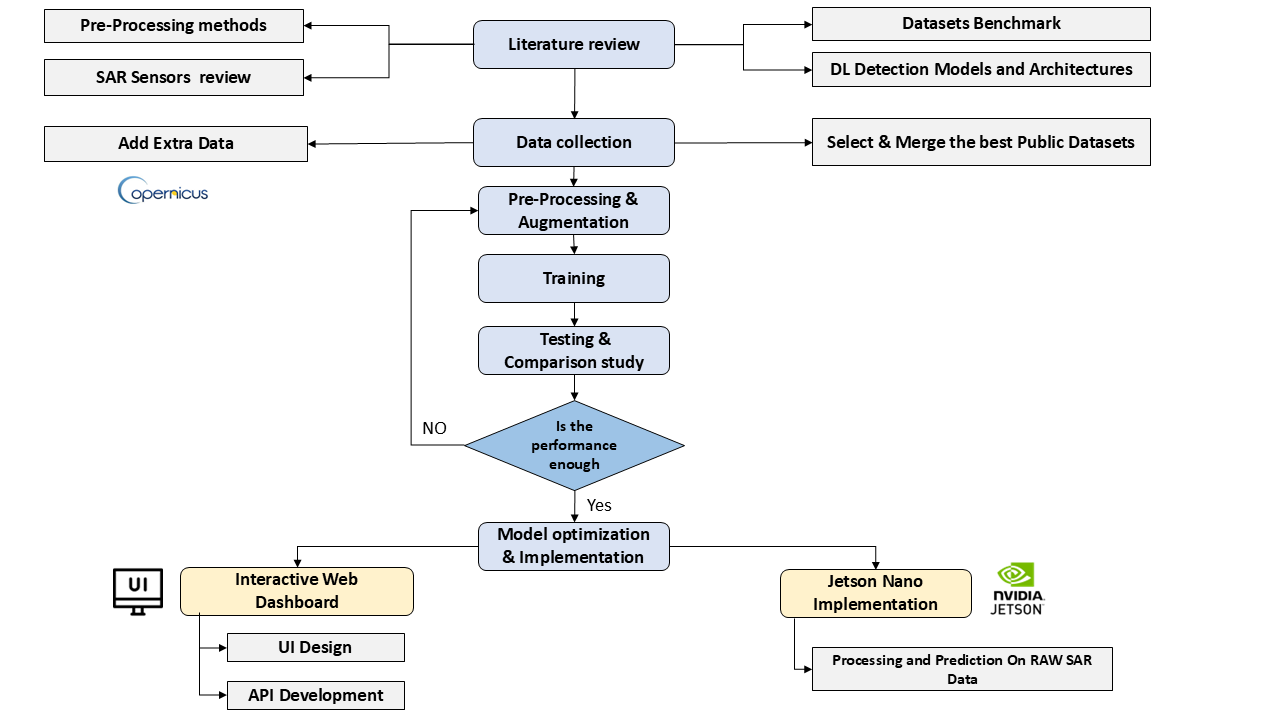
\includegraphics[width=1\linewidth]{flow.png}
    \caption{High Level System Architecture Flowchart}
    \label{fig:high_level_architecture}
\end{figure}

\subsection{Detailed Component Design}
\subsubsection{Data Acquisition and Management}
The data acquisition algorithm for the \acrshort{sar} ship detection project involves a systematic selection and integration of publicly available datasets from diverse sources, including Kaggle, GitHub, and Roboflow, to construct a robust training dataset.\\

Initially, a screening process identified two prominent public datasets: the \acrshort{sar}-Ship Dataset, comprising 43,819 images (10,2 Gaofen-3 and 10,8 Sentinel-1) with a resolution of 3–25 m, containing 59,535 ship instances of 256 × 256 pixels, and the \acrshort{ssdd} (\acrshort{sar} Ship Detection Dataset), consisting of 1,160 images from Sentinel-1, RadarSat-2, and TerraSAR-X with 1–15 m resolution, featuring 2,358 ship instances of 500 × 500 pixels. These datasets were merged to form a unified corpus; however, a critical deficiency in \acrshort{vv} polarization highly effective for detecting metallic surfaces was identified. To address this, additional data were downloaded from Copernicus, and the SNAP software was employed to extract \acrshort{vv} bands, exporting them as PNG files. \\

Subsequently, the \acrshort{ais} \acrshort{api} was utilized to enable automated labeling, enhancing dataset accuracy. Finally, these enriched data were integrated to yield a final dataset encompassing multiple bands and resolutions, optimized for advanced ship detection and tracking applications. \begin{figure}[!ht]
    \centering
    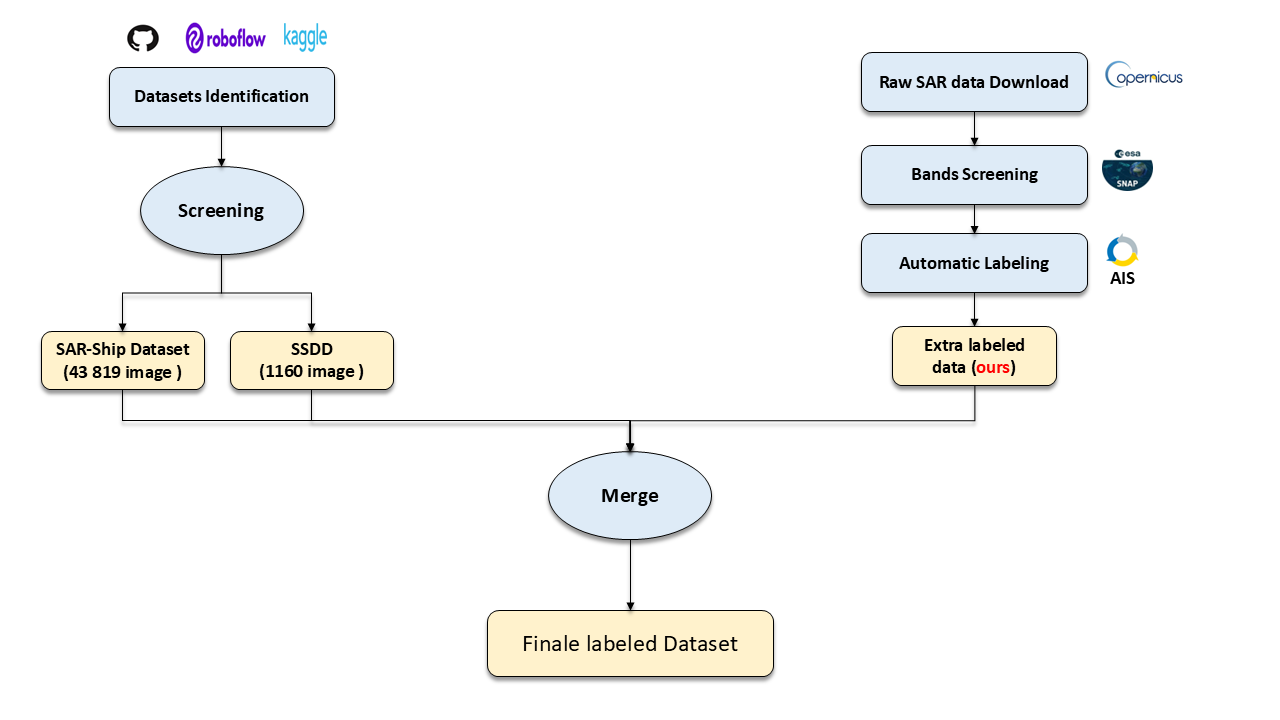
\includegraphics[width=1\linewidth]{dataacqui.png}
    \caption{Data Acquisition Flowchart}
    \label{fig:data_acquisition}
\end{figure}
\subsubsection{Preprocessing Subsystem}
Accurate ship detection in Synthetic Aperture Radar (\acrshort{sar}) imagery is highly dependent on robust preprocessing techniques that enhance discriminative features while mitigating noise, clutter, and irrelevant background information. \acrshort{sar} images present unique challenges, including speckle noise, low contrast in certain sea conditions, and interference from land areas, which necessitate a carefully designed preprocessing pipeline. The following steps are applied to optimize \acrshort{sar} data for subsequent ship detection algorithms, ensuring improved target visibility and reduced false alarms. \begin{figure}[!ht]
    \centering
    
\includegraphics[width=1\linewidth]{flow_preprocessing.PNG}
    \caption{Preprocessing Subsystem Flowchart}
    \label{fig:preprocessing_flowchart}
\end{figure}
First, polarimetric band selection is performed to optimize ship-background separability. Next, Amplitude Scaling \& Grayscale Conversion is applied to enhance interpretability while preserving critical backscatter characteristics. Then, speckle reduction filters are employed to mitigate noise while preserving structural details. Finally, land masking is applied to exclude irrelevant terrestrial regions and focus processing on maritime areas. \paragraph{Band Selection}
Polarization refers to the orientation of the plane in which a transmitted electromagnetic wave oscillates. Radar can collect signals in different polarizations by controlling the analyzed polarization in both the transmit and receive paths. While the orientation can occur at any angle, \acrshort{sar} sensors typically transmit linearly polarized. The horizontal polarization is indicated by the letter H, and the vertical polarization is indicated by the letter V.\\

The advantage of radar sensors is that signal polarization can be precisely controlled on both transmit and receive. Signals emitted in vertical (V) and received in horizontal (H) polarization would be indicated \acrshort{vh}. Alternatively, a signal that was emitted in horizontal (H) and received in horizontal (H) would be indicated \acrshort{hh}, and so on. Examining the signal strength from these different polarizations carries information about the structure of the imaged surface based on the following types of scattering: rough surface, volume, and double bounce.\\

Rough surface scattering, such as that caused by bare soil or water, is most sensitive to \acrshort{vv} scattering. Volume scattering caused by the leaves and branches in a forest canopy is most sensitive to cross-polarized data like \acrshort{vh} or HVDouble bounce scattering is caused by buildings, tree trunks, or inundated vegetation and is most sensitive to an \acrshort{hh} polarized signal.\\

The selection of the \acrshort{vv} polarization band for ship detection is grounded in \acrshort{sar} physics. \acrshort{vv} backscatter is highly sensitive to metallic structures and sea surface roughness caused by ship wakes, making it ideal for distinguishing vessels from calm water. Empirical tests on the \acrshort{sar}-\acrshort{ssdd} dataset showed that raw \acrshort{vv} intensities often exhibit low contrast between ships and background clutter, particularly for small vessels (<50m). \paragraph{Amplitude Scaling \& Grayscale Conversion}
The first preprocessing step involves amplifying the \acrshort{vv}-polarized radar returns by a factor of 2. This linear scaling brightens low-intensity backscatter values, improving the visibility of subtle features such as metallic ship structures against sea clutter while maintaining relative intensity relationships. The adjustment compensates for \acrshort{sar}’s inherent dynamic range limitations, ensuring that dark, smooth sea surfaces remain distinguishable from bright, high-backscatter targets like ships.\\

\acrshort{sar} imagery captures the backscattered radar signal, which is proportional to the target’s reflectivity and surface roughness. The raw amplitude values of \acrshort{sar} data typically exhibit a wide but compressed dynamic range due to: Logarithmic Nature of Radar Backscatter and Low Signal-to-Clutter Ratio.\\

Logarithmic Nature of Radar Backscatter: The radar cross-section (\acrshort{rcs}) of maritime targets (e.g., ships) and the surrounding sea surface follows an exponential distribution, where most pixels correspond to low-intensity sea clutter, while a few bright pixels represent strong scatterers (e.g., ship superstructures).\\

Low Signal-to-Clutter Ratio (\acrshort{scr}): Ships, especially small ones, often have backscatter intensities only slightly higher than the surrounding sea, making them difficult to distinguish without contrast enhancement.\\

Linear amplitude scaling (multiplying by a factor of 2) is a simple yet effective method to improve visualization because preserve  Relative Contrast, Unlike nonlinear transformations (e.g., gamma correction), linear scaling maintains the proportionality between pixel values, ensuring that intensity relationships crucial for target discrimination remain intact. In addition increase Adaptation to Human Vision: The human eye perceives brightness logarithmically, meaning small differences in low-intensity regions are harder to detect. By amplifying the entire dynamic range linearly, subtle backscatter variations in dark areas (e.g., calm sea) become more perceptible without saturating bright targets.\\

The 2× scaling enhances the interpretability of \acrshort{sar} imagery by: Accentuating Ship Signatures (Metallic structures and complex geometries on ships produce stronger backscatter, which becomes more pronounced after scaling) and Suppressing Noise in Dark Regions (Smooth sea surfaces (low backscatter) appear brighter, reducing the risk of false negatives in low-contrast conditions).\\

Linear scaling by a factor of 2× was chosen after evaluating three scaling factors (1.5×, 2×, 3×) on a validation set of 200 Sentinel-1 images. The Contrast-to-Noise Ratio (CNR) was used as the metric:
$$CNR = \frac{|\mu_{\text{ship}} - \mu_{\text{sea}}|}{\sqrt{\sigma_{\text{ship}}^2 + \sigma_{\text{sea}}^2}}
$$
Results showed that 2× scaling maximized CNR (improvement of $\sim 35\%$ over unscaled data) without saturating pixel values (Table \ref{tab:cnr_fp}). Higher factors (e.g., 3×) introduced artifacts in high-backscatter regions (e.g., wave fronts), degrading detection accuracy. \begin{table}[h]
\centering
\begin{tabular}{ccc}
\hline
Scaling Factor & CNR (dB) & False Positives/km² \\
\hline
1.5$\times$ & 12.7 & 1.2 \\
2.0$\times$ & 15.3 & 0.8 \\
3.0$\times$ & 14.1 & 1.5 \\
\hline
\end{tabular}
\caption{CNR and False Positives at Different Scaling Factors}
\label{tab:cnr_fp}
\end{table}


Following amplification, the adjusted \acrshort{vv} channel is duplicated across all three RGB channels to produce a grayscale representation. This conversion aligns with conventional \acrshort{sar} visualization practices, eliminating potential color-induced bias and maximizing contrast for backscatter variations. Since ship detection often relies on textural and geometric differences, grayscale rendering ensures optimal clarity for both human analysts and algorithmic processing.\\

Backscatter Intensity is used as Primary Discriminant, because in \acrshort{sar} imagery, the \acrshort{vv} (vertical-vertical) polarization channel is particularly sensitive to surface roughness and vertical structures, making it ideal for ship detection. Ships typically exhibit stronger backscatter than the surrounding sea due to their metallic composition and complex geometry. Grayscale representation preserves the absolute intensity values of the \acrshort{vv} channel, which directly correlate with radar cross-section (\acrshort{rcs}) and are critical for distinguishing targets from clutter.\\

Unlike optical imagery, \acrshort{sar} data does not inherently contain spectral (color) information. False-color composites, while sometimes used for multi-polarization data, can introduce perceptual bias without adding meaningful discriminative features for single-channel (\acrshort{vv}) ship detection. Grayscale eliminates the risk of misleading color mappings, ensuring that intensity variations are interpreted consistently.\\

\paragraph{Noise Reduction and edge enhancing}
This part of the preprocessing is aimed at removing the noise of the \acrshort{sar} image and enhancing the shape of the ships. The reason we do this step is for minimizing the chance of false negatives by making sure the AI doesn’t get confused by the noise and making the ship shapes more enhanced. This transformation adds a gamma filter with gamma value 0.6 and after that an enhancing filter with an alpha of 10/7 or 1.4285714285714.\\

Because the ships on the \acrshort{sar} images with the \acrshort{vv} polarization are really bright, that means if we reduce greatly the light of the image, the ships will still be visible, but the noise, which is less bright than the ships, will be reduced so much, that it will get a color value of 0, making the noise completely disappear, leaving only the more brighter objects behind (aka. the ships). We do that by applying a gamma correction filter with a gamma value of 0.6, which reduces the color of the image enough so that it doesn’t remove details from the ships, but removes the noise. After that some noise may still be present, but the image needs to be brighter and if we make it brighter with the gamma correction filter, the remaining noise will also get brighter. That’s why we run an image enhancing filter, which makes the brighter objects even brighter and the dimmer objects - not so much, which means if there is remaining noise there, it will be very dim. After all of that the result should look like Figure~\ref{fig:noise_reduction_comparison}. Gamma correction on \acrshort{sar} (Synthetic Aperture Radar) images is a technique used to adjust the contrast of the images without changing their average brightness. This helps in enhancing image details and making features more distinguishable visually. Specifically, gamma correction modifies the pixel intensity values according to a nonlinear curve to improve the visibility of areas that are either too dark or too bright in the original \acrshort{sar} images \cite{10.1117/12.3054990}. \begin{figure}[!ht]
    \centering
    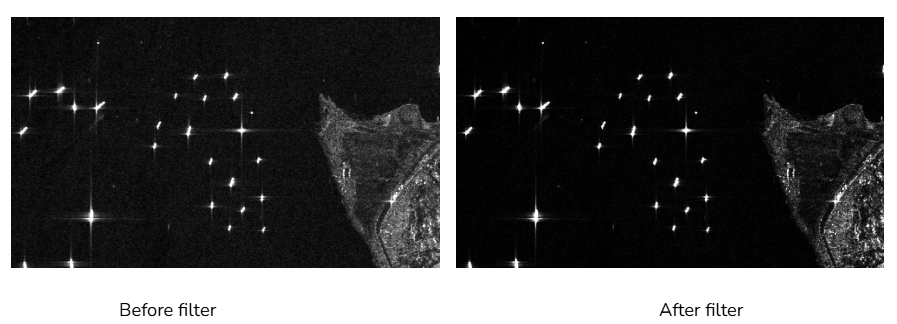
\includegraphics[width=0.7\linewidth]{image.png}
    \caption{Before \& After: Noise Reduction \& Edge Enhancement}
    \label{fig:noise_reduction_comparison}
\end{figure}

The mathematical theory of gamma correction is based on a nonlinear power-law function that adjusts the luminance or pixel intensity values of images to compensate for the nonlinear response of display devices or to enhance image contrast. Formally, gamma correction is expressed by the equation:
$$V_{out}=A \cdot V_{in}^\gamma$$
where:
\begin{itemize}
    \item $V_{in}$ is the input pixel intensity or luminance, typically normalized between 0 and 1,
    \item $\gamma$ (gamma) is the non-negative real number exponent,
    \item A is a scaling constant
    \item $V_{out}$  is the gamma-corrected output intensity. \end{itemize}
The exponent  $\gamma$ governs the shape of the curve:
\begin{itemize}
    \item If  $\gamma<1$, the function expands the dark tones and compresses highlights, effectively brightening the image (gamma compression or encoding). \item If $\gamma>1$, it reduces the dark tones and expands highlights, darkening the image (gamma expansion or decoding). \end{itemize}

\paragraph{Land Masking}
The final step in the preprocessing pipeline for ship detection in \acrshort{sar} images is land segmentation, which aims to separate land areas from water bodies to reduce false positives in ship detection. The implemented approach consists of several stages, combining advanced image processing techniques to achieve robust land masking. In \acrshort{sar}-based land-water segmentation, the primary objective is robust separation of terrestrial and aquatic regions not the preservation of fine details such as ship signatures or wave textures. However, this task is complicated by speckle noise, an inherent granular distortion in \acrshort{sar} imagery caused by coherent radar wave interference. Unlike additive noise, speckle is multiplicative, meaning it scales with local backscatter intensity, obscuring true land-water boundaries. While conventional filters (e.g., Gaussian blur) indiscriminately smooth noise and edges alike, the Lee filter excels by adaptively suppressing speckle while preserving critical structural features like coastlines. \subparagraph{Lee filter}
The Lee filter operates by analyzing local statistics within a sliding window (e.g., 35×35 pixels). It first computes the local mean ($\mu$) and variance ($\sigma^2$), deriving the coefficient of variation ($CV = \frac{\sigma}{\mu}$) to distinguish homogeneous regions (e.g., open water) from edges (e.g., land-water transitions). In low-CV areas (indicative of uniform backscatter, such as calm water), the filter aggressively smooths noise. In high-CV regions (suggesting edges), it preserves pixel values to maintain boundary sharpness. The filter’s weighting mechanism ensures that pixels near strong edges remain largely unaltered. The weighting factor, $W =\frac{1}{(1 + k·CV²)}$, balances smoothing intensity, where a higher $k$ increases denoising strength. This adaptability prevents the excessive blurring typical of median or mean filters, which might otherwise erode critical coastline features.\\

Unlike non-local or deep learning-based denoising methods, the Lee filter is computationally lightweight, making it suitable for large-scale \acrshort{sar} processing pipelines where rapid land masking is essential.\\

By selectively smoothing speckle in homogeneous water regions while retaining edge integrity, the Lee filter produces an image optimized for threshold-based segmentation. Water areas appear more uniform, reducing false positives during binarization, while coastlines remain sharply defined. Subsequent steps such as flood-filling and contour filtering benefit from this preprocessing, as the filter’s output minimizes artifacts that could propagate errors into the final land mask. Thus, the Lee filter serves as a foundational step in \acrshort{sar} land-water segmentation, striking an optimal balance between noise suppression and feature preservation. \begin{figure}[!ht]
    \centering
    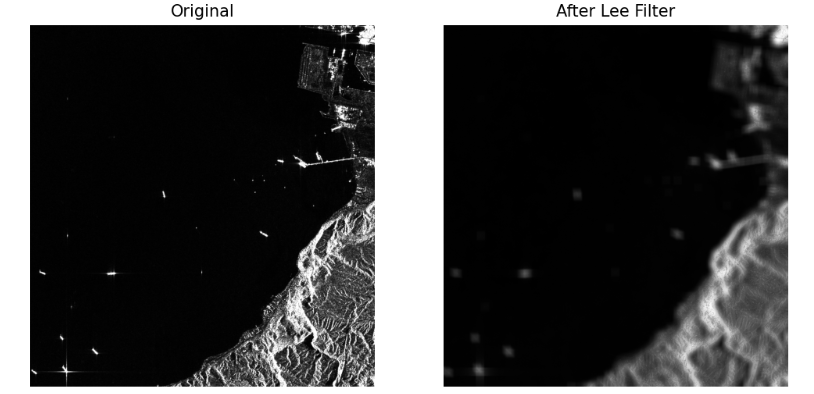
\includegraphics[width=0.75\linewidth]{Lee_filter.png}
    \caption{Before \& After: Lee filter Application}
    \label{fig:lee_filter_comparison}
\end{figure}

\subparagraph{Multi-stage Denoising}
Before performing land segmentation on \acrshort{sar} (Synthetic Aperture Radar) images, in order to detect land more easily is crucial to reduce noise and enhance relevant features while preserving structural details. A multi-stage denoising and enhancement approach is applied, consisting of Gaussian Blurring for Noise Reduction and Contrast-Limited Adaptive Histogram Equalization (CLAHE). The theoretical basis of Gaussian blurring for noise reduction lies in its role as a low-pass filter implemented by convolution with a Gaussian function a bell-shaped curve defined by the Gaussian distribution. This approach smooths an image by replacing each pixel’s value with a weighted average of its neighbors, where the weights are given by the Gaussian function. The Gaussian assigns higher weights to pixels closer to the center and lower weights to pixels farther away, creating a smooth, natural blur that reduces high-frequency noise while preserving important image details and edges better than uniform averaging filters. Mathematically, the Gaussian function in two dimensions is the product of two 1D Gaussians:$$G(x, y) = \frac{1}{2\pi\sigma^2} e^{-\frac{x^2 + y^2}{2\sigma^2}}$$
where x and y are distances from the center pixel horizontally and vertically, and $\sigma$ (sigma) is the standard deviation that controls the amount of blur. Convolution with this kernel results in smoothing by effectively attenuating high-frequency components such as random noise, while preserving lower-frequency components related to the image’s underlying structure. \\


The theoretical basis of Contrast-Limited Adaptive Histogram Equalization (CLAHE) lies in its enhancement of image contrast by performing localized histogram equalization with a mechanism to limit contrast amplification and prevent noise over-amplification. Instead of applying histogram equalization globally on the entire image, CLAHE divides the image into smaller local regions (tiles or blocks) and enhances contrast within each of these regions independently. This allows CLAHE to improve local details and contrasts that global histogram equalization might miss or wash out. In basic Adaptive Histogram Equalization (AHE), the contrast can be overly amplified in nearly homogeneous regions, because the local histogram in such regions is highly peaked, which leads to noise amplification. CLAHE addresses this by clipping the histogram at a predefined threshold called the clip limit. Histogram bins exceeding this clip limit are clipped, and the excess is redistributed across all histogram bins. This limits the slope of the cumulative distribution function (CDF) used for equalization, effectively capping the maximum contrast enhancement and reducing noise amplification in smooth regions. \begin{figure}[!ht]
    \centering
    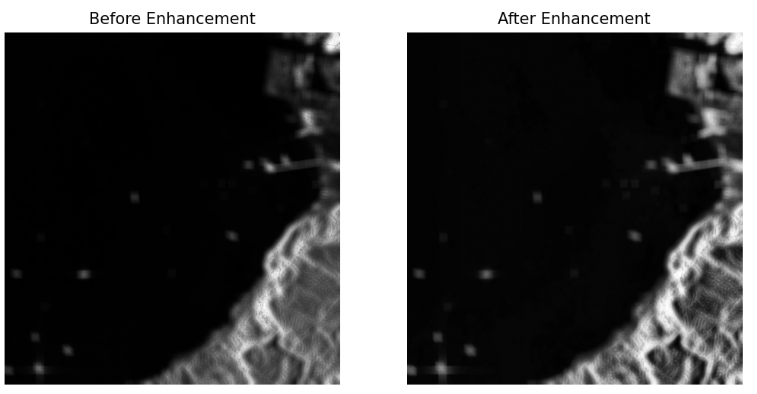
\includegraphics[width=0.75\linewidth]{denoising.png}
    \caption{Before \& After: Multi-stage Denoising}
    \label{fig:denoising_comparison}
\end{figure}
\subparagraph{Combined Thresholding}
After denoising and contrast enhancement, the next critical step is thresholding, which converts the grayscale image into a binary mask where land and water regions are separated. Since \acrshort{sar} images exhibit varying backscatter intensities due to terrain roughness, a single thresholding method may fail to capture all land areas accurately. To address this, two complementary thresholding techniques are applied:
\begin{itemize}
    \item Otsu’s Global Thresholding (for coarse separation)
    \item Adaptive Gaussian Thresholding (for local variations)
\end{itemize}
The results are then combined to ensure robust land detection \cite{4310076}. \\

\textbf{Otsu thresholding} is based on finding an optimal threshold that separate an image into two classes (background and foreground) by minimizing the within-class variance or equivalently maximizing the between-class variance of pixel intensities. Let an image have \( L \) discrete intensity levels \(\{0, 1, ..., L - 1\}\), with normalized histogram probabilities \( p_i \) representing the fraction of pixels at intensity level \( i \). So, \(\sum_{i=0}^{L-1} p_i = 1\).

Select a threshold \( t \) that divides pixels into two classes:

\begin{itemize}
    \item \( C_1 \) with intensities \(\{0, ..., t\}\)
    \item \( C_2 \) with intensities \(\{t + 1, ..., L - 1\}\)
\end{itemize}

Class probabilities are:

\[
\omega_1(t) = \sum_{i=0}^t p_i, \quad \omega_2(t) = \sum_{i=t+1}^{L-1} p_i = 1 - \omega_1(t)
\]

Class means (average intensities):

\[
\mu_1(t) = \frac{\sum_{i=0}^t i p_i}{\omega_1(t)}, \quad \mu_2(t) = \frac{\sum_{i=t+1}^{L-1} i p_i}{\omega_2(t)}
\]

The total mean intensity of the image is:

\[
\mu_T = \sum_{i=0}^{L-1} i p_i
\]

The within-class variance (weighted sum of variances of the two classes) is:

\[
\sigma_w^2(t) = \omega_1(t) \sigma_1^2(t) + \omega_2(t) \sigma_2^2(t)
\]

where \(\sigma_1^2(t)\) and \(\sigma_2^2(t)\) are variances of the classes.\\

Otsu's method chooses the threshold \( t^* \) that minimizes \(\sigma_w^2(t)\). Equivalently, because the total variance \(\sigma_T^2\) is constant for the image, minimizing within-class variance is the same as maximizing the between-class variance:

\[
\sigma_b^2(t) = \omega_1(t) \omega_2(t) [\mu_1(t) - \mu_2(t)]^2
\]

The optimal threshold \( t^* \) satisfies:

\[
t^* = \arg \max_t \sigma_b^2(t)
\]

This approach finds the threshold that best separates the intensity histogram into two classes with maximal distinction between their means, giving effective segmentation especially for bimodal histograms.\\

\textbf{Adaptive Gaussian Thresholding} is a local image binarization technique where the threshold value varies across the image depending on the local pixel intensities. Instead of using a single global threshold for the entire image, it calculates a threshold for each pixel based on a weighted average of the surrounding pixel values in a local neighborhood. The weights follow a 2D Gaussian distribution centered on the pixel, emphasizing closer pixels more heavily. The local threshold is computed as this Gaussian-weighted mean minus an offset constant. Pixels brighter than this threshold are set to one value (e.g., white), and others to another (e.g., black), effectively segmenting the image. This approach is especially useful for images with uneven lighting or backgrounds.\\

In mathematical terms, for each pixel, the threshold T is: $$T=\text{Gaussian weighted average of pixels in the neighborhood}-\text{offsetT}$$ weighted average of pixels in the neighborhood offset

The local neighborhood is typically a square block around the pixel, defined by the kernel size. The pixel values within this block are averaged with Gaussian weights, providing a smooth, locally adaptive threshold surface. The offset shifts the threshold up or down relative to this local mean to better segment the object of interest. This method handles spatial variations in illumination better than global thresholding. \begin{figure}[!ht]
    \centering
    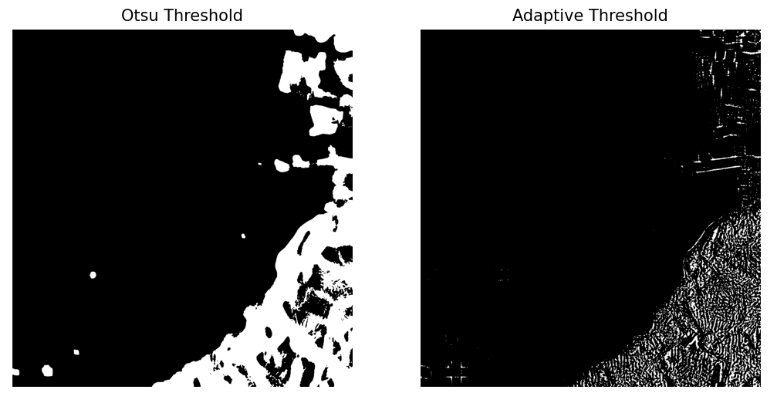
\includegraphics[width=0.75\linewidth]{Threshold.png}
    \caption{Application of Thresholds}
    \label{fig:threshold_comparison}
\end{figure}

\subparagraph{Morphological Processing}
After thresholding, the binary mask may still contain imperfections, such as: Small gaps in land regions (due to texture variations or noise) and Isolated noise pixels (misclassified as land or water). These imperfections can create problems when creating a land mask.

To address these issues, morphological operations are applied. These operations modify the binary mask using a structuring element (a small predefined shape) to enhance the land segmentation.\\

Morphological processing is a set of image processing operations that work on the shape of objects within binary images (images with pixels valued 0 or 1, e.g., background and foreground). In the context of refining a binary mask, two key morphological operations are the closing and opening operations. The purpose of Closing Operation is To fill small gaps or holes inside the foreground (land) regions of the binary mask. It smooths the boundaries by closing narrow breaks or thin black points (holes). The Process consist in
\begin{itemize}
    \item Dilation: Expands the white (foreground) regions, causing small holes or gaps to shrink or disappear by growing the object boundaries. \item Erosion: Shrinks the expanded region back to approximately the original size but without the small holes filled. \end{itemize}
In this way, Small holes and gaps inside land regions are effectively filled without significantly altering the size or shape of larger regions.\\


The purpose of Opening Operation is To remove small noise or artifacts (small white spots or tiny land regions) from the binary mask while preserving the size and shape of the main land regions. Process:
\begin{itemize}
    \item Erosion: Shrinks the white (foreground) regions, removing small objects or protrusions completely if they are smaller than the structuring element. \item Dilation: Grows the eroded regions back to close to their original size, but small noises removed by erosion do not come back. \end{itemize}
As effect, Small isolated noise pixels or thin connections are eliminated, smoothing the shape of the remaining landmasses. \begin{figure}[!ht]
    \centering
    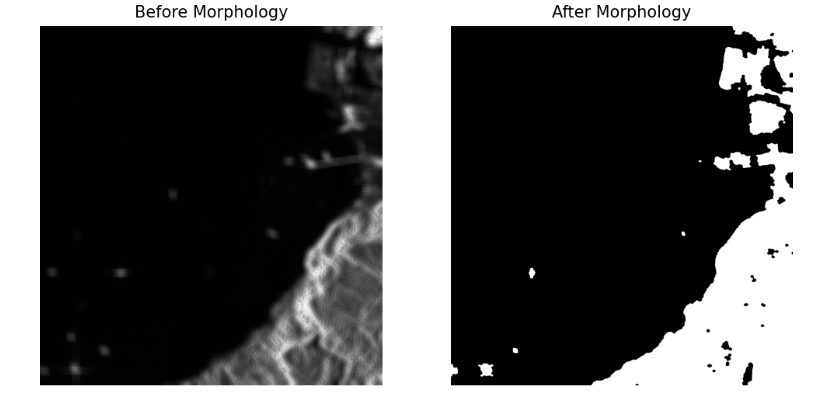
\includegraphics[width=0.75\linewidth]{Morph.png}
    \caption{Before \& After: Morphological Processing}
    \label{fig:morph_comparison}
\end{figure}

\subparagraph{Flood-Filling for Background Removal}
Flood-filling plays a crucial role in refining the land mask by ensuring accurate separation between water and land regions. While thresholding and morphological operations provide an initial segmentation, they may leave residual noise or misclassified pixels, particularly near image borders and complex coastal areas. Since water bodies in \acrshort{sar} imagery are expected to form continuous regions, flood-filling from predefined seed points (typically image corners, assumed to be water) helps propagate a consistent background label across all connected water pixels. This step effectively corrects discontinuities caused by noise or thresholding artifacts, producing a more coherent mask. The resulting flood-filled region is then inverted to isolate land areas, ensuring that only true terrestrial structures remain for subsequent analysis. This method enhances segmentation robustness, minimizing false positives in ship detection by reliably excluding water-dominated regions.\\

The algorithm operates by selecting seed points typically at image corners under the assumption that they represent water and propagating labels through connected regions based on either 4-way (direct adjacency) or 8-way (including diagonals) pixel connectivity. This region-growing approach systematically identifies all contiguous background (water) pixels through iterative traversal, such as breadth-first search (BFS), ensuring computational efficiency even for large images. Once completed, the resulting mask is inverted to isolate land areas, transforming initially marked water regions (0) into background and preserving unmarked pixels (1) as foreground land. This process corrects common artifacts from thresholding, such as fragmented water bodies or misclassified coastal pixels, by enforcing spatial continuity in the background.\\

Mathematically, if M denotes the binary mask and S the seed set, flood filling of all $p \in  S$ where $M(p) = 0$ guarantees comprehensive extraction of the water region. The inversion, $M \leftarrow 1 - M$, then produces a final mask where land is distinctly separated, enhancing downstream ship detection accuracy by eliminating residual noise and edge discontinuities. The method’s efficacy hinges on the strategic selection of seed points and connectivity rules, balancing precision with computational tractability. \subparagraph{Contour Filtering}
Following flood-filling, the generated binary land mask often contains residual artifacts that require further processing to ensure segmentation accuracy. These artifacts typically manifest as small false-positive regions such as speckle noise misclassified as land or genuine but insignificant features like tiny islets which are irrelevant for ship detection purposes. \\

To address this, contour filtering is employed as a critical refinement step. The process involves detecting all connected components in the binary mask through contour analysis, then applying size-based filtering to retain only meaningful landmasses. By establishing an area threshold (typically determined through empirical analysis of the specific \acrshort{sar} dataset), small contours below this threshold are systematically removed. \\

This operation effectively eliminates noise while preserving cartographically significant coastal and inland features. The resulting refined mask provides a more accurate representation of land areas, thereby reducing false alarms in subsequent ship detection phases. This approach demonstrates how morphological post-processing can enhance segmentation quality by incorporating domain-specific knowledge about the expected scale of relevant land structures in maritime surveillance scenarios. \begin{figure}[!ht]
    \centering
    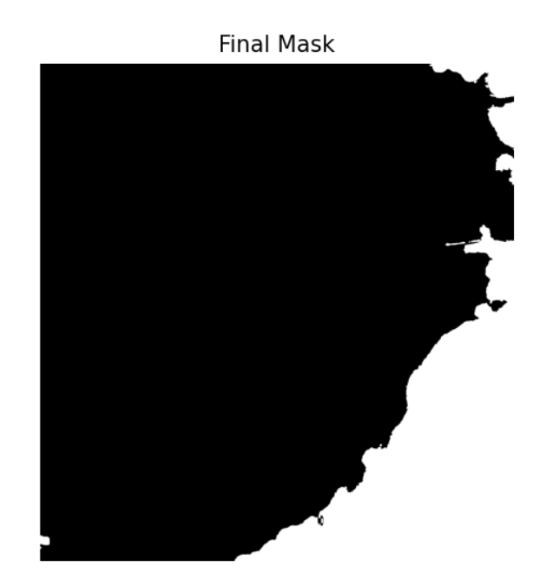
\includegraphics[width=0.4\linewidth]{mask.png}
    \caption{Final Mask Obtained}
    \label{fig:final_mask}
\end{figure}

\subparagraph{Iterative Refinement \& Final Output}
The inherent complexity of \acrshort{sar} imagery characterized by intricate coastal geometries, archipelagos, and heterogeneous backscattering often necessitates an iterative approach to land segmentation. A single pass of land masking may prove insufficient, as residual artifacts or misclassified regions can persist, particularly in challenging environments. To address this, an adaptive refinement process is implemented, which evaluates and progressively improves the segmentation quality through successive iterations.\\

The algorithm first assesses the initial land mask by computing the percentage of land pixels relative to the total image area. This metric serves as a critical indicator of segmentation validity: if the land coverage exceeds 85\%, the scene is deemed predominantly terrestrial and thus unsuitable for maritime ship detection, resulting in discarding the image. Conversely, if land occupies more than 15\% of the image, the system proceeds with refinement. In such cases, targeted denoising and secondary masking are applied to eliminate false positives, such as speckle noise misinterpreted as small islands or fragmented coastal artifacts. Each iteration recalculates the land percentage, ensuring convergence toward an optimal mask where only cartographically relevant landmasses are preserved.\\

This iterative framework not only enhances robustness in diverse geographical contexts but also automates the trade-off between over-segmentation (excessive land removal) and under-segmentation (inadequate noise suppression). By dynamically adjusting to scene-specific characteristics, the method ensures reliable land masking, which is foundational for accurate ship detection in operational \acrshort{sar} analysis pipelines. \begin{figure}[!ht]
    \centering
    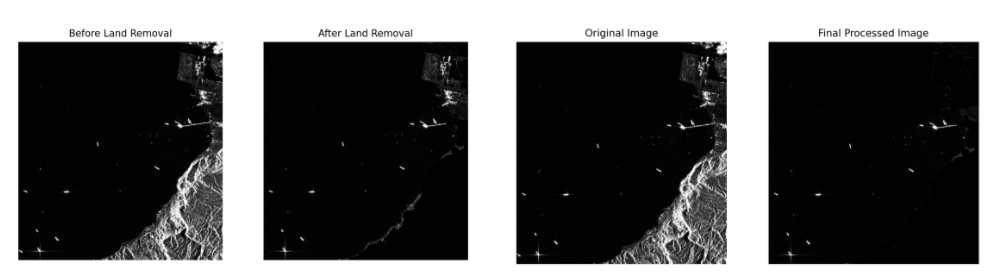
\includegraphics[width=1\linewidth]{masking.png}
    \caption{Comparization between Original Image and Resuts of first ans second preprocessing iteration}
    \label{fig:masking_iteration_comparison}
\end{figure}

\subsubsection{Machine Learning Detection Model}
The performance comparison graph provided by Ultralytics, which plots mean average precision (\acrshort{map}) at IoU thresholds from 0.5 to 0.95 against latency in milliseconds per image on a T4 \acrshort{tensorrt} FP16 platform (Figure \ref{fig:performance_comparison_graph}), serves as a critical diagnostic tool for evaluating candidate models for our \acrshort{sar}-based ship detection and tracking project.\\

Analyzing the graph reveals that YOLOv11n achieves a modest 40\% \acrshort{map} with a latency of 2-3 milliseconds, indicating high speed but insufficient precision for detecting small ships in \acrshort{sar} imagery, where targets often occupy a tiny fraction of the image. \begin{figure}
    \centering
    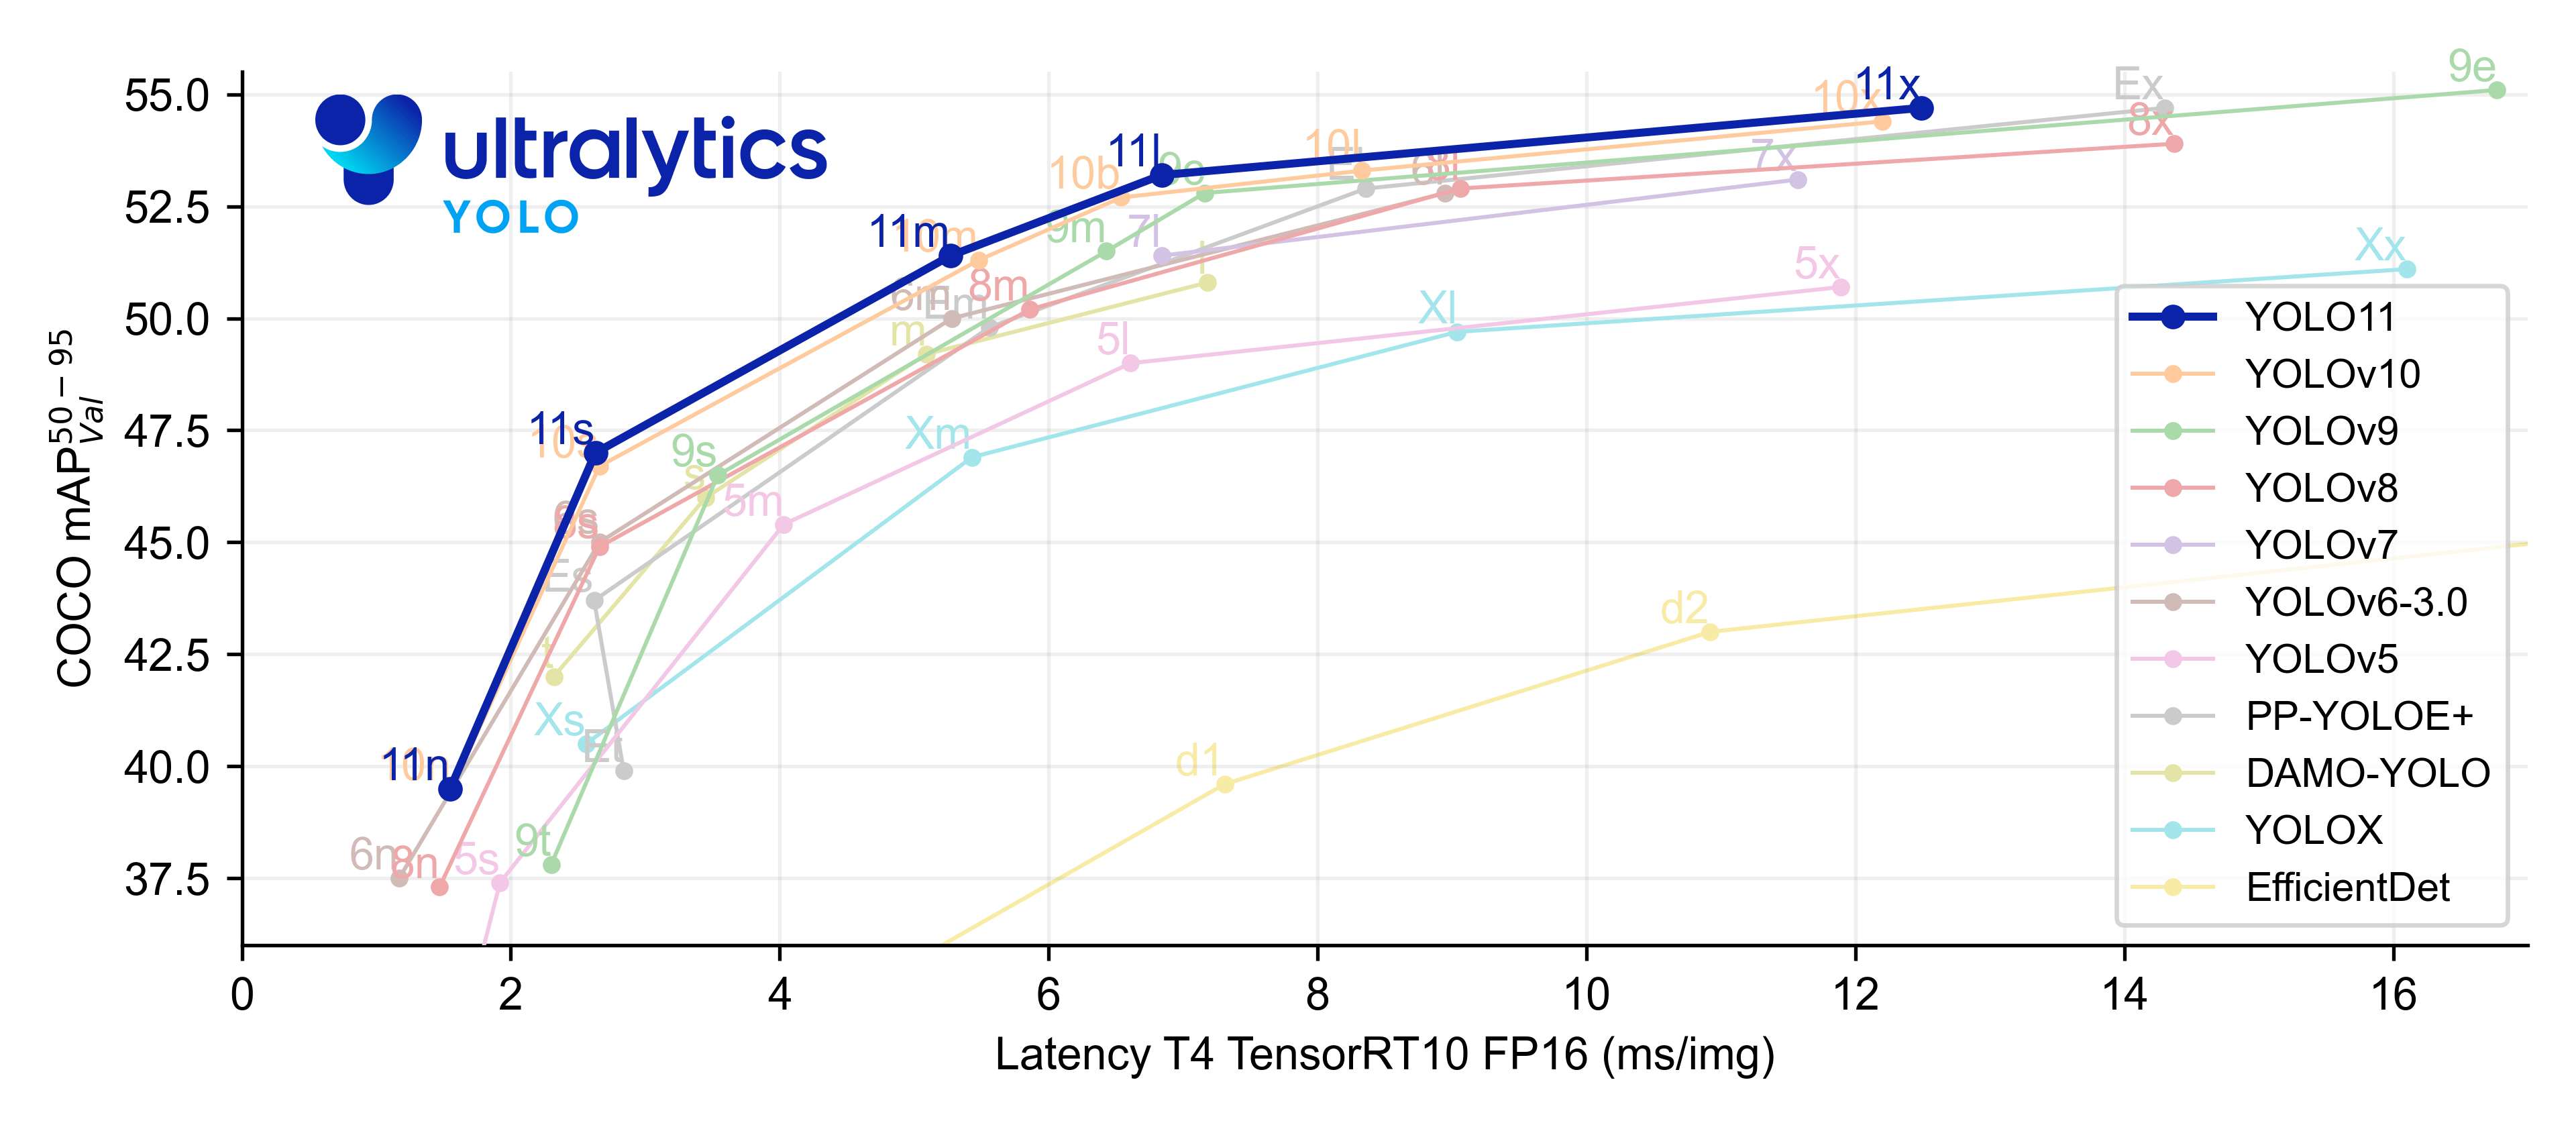
\includegraphics[width=0.75\linewidth]{performance-comparison.png}
    \caption{Performance Comparison Graph}
    \label{fig:performance_comparison_graph}
\end{figure}
YOLOv11l, while offering a higher \acrshort{map} of 54\% with 8 milliseconds latency, exceeds the computational capacity of the resource-constrained NVIDIA Jetson Nano, a low-power edge device with a 128-core Maxwell GPU, making it impractical for real-time deployment. YOLOv8m and YOLOv10m, with \acrshort{map} values of 46\% and 50\% respectively and latencies around 6 milliseconds, provide moderate performance but fall short in precision for small-object detection and remain borderline for Jetson Nano compatibility.\\

In contrast, \acrshort{yolov11m} emerges as the optimal choice, delivering a balanced 52.5\% \acrshort{map} with a latency of 4-5 milliseconds, which aligns with the project’s dual requirements of high precision for small ship detection and efficient operation on limited hardware. This model’s architectural enhancements, likely including improved feature pyramid networks or anchor-free detection heads, enhance its ability to capture fine details in \acrshort{sar} images, as evidenced by its superior \acrshort{map} compared to predecessors.\\

Furthermore, with optimizations reducing memory usage and accelerating inference up to 4x it can achieve real-time processing rates of 10-20 frames per second on the Jetson Nano, as supported by studies like \cite{rasheed2025yolov11} on edge optimization of YOLO models and \cite{en15238816} on efficient neural networks, solidifying \acrshort{yolov11m} as the best fit for our maritime surveillance application. \subsection{Tracking Algorithm}
The tracking component of the ship detection system will leverage advanced multi-object tracking methodologies to ensure robust performance across dynamic maritime environments, requiring multiple sequential images to enable consistent tracking over time. Techniques such as \acrshort{deepsort}, a deep learning-enhanced extension of the SORT algorithm, will be considered, integrating detection outputs from \acrshort{yolov11m} with temporal association and appearance features to maintain consistent tracking IDs across frames. This approach will employ a Kalman filter for motion prediction and a deep association metric, potentially utilizing convolutional neural networks, to handle occlusions and re-identification challenges inherent in \acrshort{sar} imagery. Additionally, fusion with \acrshort{ais} data will enhance tracking accuracy by correlating positional updates, ensuring real-time applicability. \subsubsection{Output and Visualization}
The visualization component will be implemented through a comprehensive Streamlit-based
dashboard, designed to provide an intuitive and interactive interface for users to engage with
the \acrshort{sar}-based ship detection system. Users will have the flexibility to upload \acrshort{sar} images
manually or automate the process by integrating with Google Earth Engine, enabling seamless
data acquisition and preprocessing tailored to specified regions of interest. Upon processing
through our algorithms, the system will generate a global output image annotated with unique
identification numbers assigned to each detected ship, alongside individual images for each ship instance, facilitating detailed analysis. Additionally, the dashboard will present statistical
insights, including the total number of detected ships, their estimated sizes in meters derived
from \acrshort{sar} resolution data, and other relevant metrics, all of which can be downloaded by users
in customizable formats (e.g., CSV, JSON, PNG) based on their preferences. The system will be
developed as a complete ecosystem, incorporating an \acrshort{api} for real-time \acrshort{ais} data integration to
enhance tracking accuracy, alongside cloud-based storage and processing capabilities to
ensure scalability and accessibility for operational maritime surveillance applications. \subsection{Data Flow and Workflow}
This section provides a detailed, step-by-step explanation of the data pipeline within the \acrshort{sar} Ship Detection system, elaborating on the high-level architecture presented previously. It provides an overview of the solution implementation and describes the processes that each stage goes through from raw \acrshort{sar} data ingestion to the final output of detected and tracked ships.\\

The data flow within the \acrshort{sar} Ship Detection Project follows a structured pipeline designed for efficiency and accuracy. The primary stages are:
\begin{itemize}
    \item \textbf{\acrshort{sar} Data Acquisition}:
    \begin{itemize}
        \item \textbf{Process}: The pipeline initiates with the acquisition of raw Synthetic Aperture Radar (\acrshort{sar}) imagery. Acquisition of data is done via the Copernicus Browser. For the hardware implementation (Jetson Nano Edge) various raw \acrshort{sar} image files are preloaded into the file system that it randomly chooses from upon use. For the cloud implementation the \acrshort{sar} data is either uploaded from the user or queried from Copernicus via user requests initiated through Google Earth. \item Details: Data can be downloaded directly from Copernicus in either raw or processed formats. Data can be in multiple file types such as .png and .jpeg as well as .tiff format which allows for use with larger image sizes through special software. The Data is uploaded to the solution via the BlueGuard website which is running the model. Data uploaded by users is first fed into a queue to ensure the page can handle the traffic. \end{itemize}
    \item \textbf{Initial Data Ingestion and Storage}:
    \begin{itemize}
        \item \textbf{Process}: Upon receiving a user request via the Streamlit web interface, the system initiates a data ingestion process that either: (1) Downloads \acrshort{sar} imagery from the Copernicus \acrshort{api} based on user-specified coordinates and time range. (2) Accepts user-uploaded \acrshort{sar} .tiff, .png, or .jpeg images directly through the web interface. (3) Finally, optionally queries \acrshort{ais} data for the corresponding area and time from a third-party \acrshort{api}. Once retrieved or uploaded, the data is temporarily stored for processing and version tracking. \item \textbf{Details}: Data is stored in local server only while in use. A structured directory or database system is utilized to manage large volumes of \acrshort{sar} images. The images once outputted to the user will be automatically deleted from the server once the unique session is over or times outs. \acrshort{sar} images and associated metadata are stored locally in a structured directory on the host laptop. Each request is isolated in a temporary directory, identified by a unique session or request ID, which avoids filename collisions and supports simple cleanup. Due to limited disk space on the host laptop, data is stored ephemerally. A background cleanup job (using a lightweight Python scheduler like APScheduler) deletes session data older than a set threshold (e.g., 15 minutes or after download). \item Each ingestion is isolated to its own session. Streamlit's session-based design supports this naturally, but in addition, image download requests are asynchronous using threads or background tasks to avoid freezing the Streamlit UI. \end{itemize}
    \item \textbf{Preprocessing Queue Management}:
    \begin{itemize}
        \item \textbf{Process}: Once a \acrshort{sar} image is ingested, it is placed in a preprocessing queue. This queue serializes and throttles incoming processing requests, ensuring that system memory and CPU/GPU resources are not overloaded when many users access the site concurrently. \item \textbf{Details}: A simple in-memory First-In-First-Out (FIFO) job queue is implemented using Python. A dedicated background worker thread or asyncio task continuously monitors the queue and processes jobs one by one. While in the queue, users are shown an estimate of their position in the queue and approximate wait time. This is implemented with Streamlit's session state and periodic UI refresh (st.experimental rerun or st autorefresh). \end{itemize}
    \item \textbf{\acrshort{sar} Image Preprocessing} (Subsystem):
    \begin{itemize}
        \item \textbf{Process}: The raw \acrshort{sar} images undergo a series of critical transformations to enhance features, reduce noise, and prepare them for machine learning inference. This stage is crucial for improving detection accuracy.
        \item \textbf{Details}:
        \begin{itemize}
            \item \textbf{Polarimetric Band Selection}
            
            Technique: \acrshort{vv} Polarization Band Selection
            
            Description: The \acrshort{vv} band is chosen due to its sensitivity to sea  surface roughness and ship wake visibility, making it ideal for ship detection.
            \item \textbf{Amplitude Scaling and Grayscale Conversion}
            
            Technique: Linear Intensity Amplification and RGB Channel Duplication
            
            Description: The \acrshort{vv} channel is amplified by a factor of 2 to improve contrast between ships and sea clutter, then converted to grayscale by copying it into all three RGB channels. \item \textbf{Noise Reduction and Edge Enhancement}
            
            Technique: Gamma Filtering and Alpha-Based Enhancement
           
            Description: A gamma correction ($\gamma = 0.6$) suppresses dim background noise while retaining ship features, followed by an enhancement filter ($\alpha = 10/7$) to increase the brightness of ships and suppress residual noise. \item \textbf{Land Masking}:
            
            Techniques: Lee Filter + CLAHE + Dual Thresholding + Morphological Processing + Flood-Fill + Contour Filtering + Iterative Refinement
        
            Descriptions:
            
            - Lee Filter: Adaptive speckle reduction filter preserves coastline boundaries while smoothing sea regions.
            
            - CLAHE: Enhances local contrast within the image while preventing over-amplification of noise. - Gaussian Blurring: Reduces high-frequency noise while preserving structure using a Gaussian convolution kernel. - Otsu's Thresholding: Global thresholding to segment land and sea by minimizing intra-class intensity variance. - Adaptive Gaussian Thresholding: Locally adaptive binarization to handle spatial variations in intensity. - Morphological Processing: Closing and opening operations correct segmentation defects (fill gaps, remove noise). - Flood-Filling: Segments water from land by propagating from known water regions (image corners), then inverts to isolate land. - Contour Filtering: Removes small false-positive land segments by filtering based on area threshold. - Iterative Refinement: Repeats segmentation and filtering until land coverage is within valid thresholds; terminates or refines further based on percentage rules (e.g., >85\% land coverage aborts detection). \item \textbf{Format Conversion and Standardization}:
            
            Technique: Conversion to \acrshort{numpy} Array and Normalization
        
            Description: The preprocessed grayscale image is converted into a normalized \acrshort{numpy} array with pixel values scaled between 0 and 1 for direct input to the deep learning model. \end{itemize}
    \end{itemize}
    \item \textbf{Ship Detection Inference} (Machine Learning Model):
        \begin{itemize}
            \item \textbf{Process}: The preprocessed \acrshort{sar} image is fed into the trained ship detection deep learning model. This model analyzes the image to identify potential ship instances. The prediction returns the annotated image and JSON file containing information regarding the ship geographical coordinates and confidence etc.
            \item \textbf{Details}: The preliminary trained model is the \acrshort{yolov11m} for its good balance of precision and latency. This model was used for preliminary analysis of the overall solution and for development of the end-to-end system. The models are trained via \acrshort{pytorch} with the respective datasets (preliminary vs final) and the weights are converted to \acrshort{onnx} format from which can be used for inference in any format, specifically \acrshort{tensorrt}, which is used for the Jetson Nano architecture. Predictions of ships are not classified into distinct ship types, the model is only trained to identify whether or not there is a ship within the data. The model is deployed on the Jetson Nano and locally on the demo website host. \end{itemize}
    \item \textbf{Output Generation}:
    \begin{itemize}
        \item \textbf{Process}: The final results, including detected ship bounding boxes, confidence scores, and unique tracking IDs, are compiled and formatted for output. \item \textbf{Details}: This output can be presented in various forms depending on the user interface:
        \begin{itemize}
            \item \textbf{Structured Data Output}: Generation of machine-readable files (JSON) containing all relevant detection and tracking metadata (coordinates, timestamps, IDs). \item \textbf{Annotated Image}: Overlaying bounding boxes, labels, and tracking IDs directly onto the original or preprocessed \acrshort{sar} imagery for visual inspection. The annotated image can be downloaded as a whole, or individual identified ships can be downloaded separately can be downloaded individually. \item \textbf{Data Downlink/Transmission}: For edge deployments (Jetson Nano), relevant output data is prepared for transmission to ground stations or other connected systems. \end{itemize}
    \end{itemize}
    \item \textbf{User Interface / Visualization}:
    \begin{itemize}
        \item \textbf{Process}: The processed results are delivered to the user through one of the defined interfaces, allowing for interaction and visualization of the detected and tracked ships. The holistic interface will be made using Streamlit and hosted as a webpage containing three pages for each sub-interface type listed below. These are different ways users can request or view use of the solution and models depending on their desired input type. \item \textbf{Details}:
        \begin{itemize}
            \item \textbf{Jetson Nano Interface}: Processed data is “downlinked” and visualized on a local display or streamed to a ground control application, potentially integrating with on-ground \acrshort{ais} data. Statistical insights are also provided. The user cannot request specific data, the jetson nano will come pre-loaded with random \acrshort{sar} image files, its functionality may be expanded once integrated into a satellite. \item \textbf{Web-based Map Interface}: Users interact with a Google Earth-style map to select a region of interest. This region of interest will be limited to a maximum size and square shape, this is to reduce the load on host machine. An \acrshort{api} fetches the latest \acrshort{sar} data, processes it and sends it to the model for prediction. The result goes through the statistical insights to be displayed to the user. \item \textbf{Image Upload Interface}: Users upload their raw \acrshort{sar} images. the system processes the image and sends it to the model for prediction. The result goes through the statistical insights to be displayed to the user. \end{itemize}
    \end{itemize}
\end{itemize}


\newpage
\section{Implementation and Development}
\subsection{Software and Hardware Environment Setup}
\subsubsection{Training Setup, Hardware + Software}
\begin{itemize}
    \item \textbf{Roboflow}
    Roboflow is a powerful, end-to-end computer vision platform that simplifies everything from dataset management and image annotation to model training and deployment. It supports over 40 data formats, offers AI-assisted labeling, and enables training with advanced architectures like YOLO. We used Roboflow to easily upload and annotate our dataset, then successfully trained a sample YOLO model within its intuitive interface. \item \textbf{Google colab}
    A versatile, cloud-based platform for writing and executing Python code in a web browser, requiring no setup. Built on Jupyter Notebook, it's a go-to tool for machine learning, data analysis, and education, offering access to powerful GPUs and TPUs. We leveraged Colab for various data processing tasks and to efficiently train our model, evaluating its suitability for our project in a streamlined, collaborative environment. \item \textbf{NVIDIA Jetson Nano}
     A compact, energy-efficient edge AI device ideal for on-orbit inference and data downlink in resource-constrained settings. Featuring a quad-core ARM CPU, 128-core Maxwell GPU, and 4 GB RAM, it supports real-time deep learning tasks like object detection and segmentation. Compatible with AI frameworks like TensorFlow, the Jetson Nano enables onboard data analysis, reducing raw data transmission and improving bandwidth efficiency perfect for autonomous, AI-driven space applications. \item \textbf{GitHub}:
    Aweb-based platform for version control and collaborative software development, built around Git. We utilized GitHub to host our project's codebase, facilitating seamless collaboration among team members and ensuring proper version control throughout the development lifecycle. \item \textbf{STREAMLIT}: an open-source Python library that simplifies the creation of custom web applications for machine learning and data science. We employed Streamlit to develop an intuitive user interface for our project, allowing for easy interaction with our trained models and visualization of results. \end{itemize}

\subsubsection{Implementation Hardware/Edge}
The primary hardware utilized for edge deployment and development in the \acrshort{sar} Ship
Detection Project is the NVIDIA Jetson Nano. Its specifications are detailed as follows:
\begin{itemize}
    \item Model: NVIDIA Jetson Nano Developer Kit (4GB version)
    \item GPU: NVIDIA Maxwell architecture with 128 NVIDIA \acrshort{cuda} cores
    \item CPU: Quad-core ARM Cortex-A57 MPCore processor @ 1.43 GHz
    \item Memory (RAM): 4 GB 64-bit LPDDR4 @ 1600MHz (25.6 GB/s bandwidth)
    \item Storage: microSD card slot (user-supplied for OS and data storage)
    \item Power Input: 5V 4A via DC barrel jack (recommended for full performance)
\end{itemize}

\subsubsection{Operating System and Core Software Versions}
\begin{itemize}
    \item Ubuntu 24.04 \acrshort{lts}
    \item Python version 3.8.10
    \item NVIDIA JetPack 4.6.1
    \item \acrshort{cuda} 10.2
    \item \acrshort{cudnn} 8.0.5
    \item \acrshort{tensorrt} 10.13.0
\end{itemize}

\subsubsection{Dependency Management and Virtual Environment Setup}
TODO

\subsubsection{Accessing the Jetson Nano}
To ssh to the Jetson Nano use:
\begin{lstlisting}
ssh jetson@<nano_ip_address>
\end{lstlisting}
\subsubsection{Essential Command Line Commands}
\begin{itemize}
    \item \textbf{\lstinline|jtop|}: (After \lstinline|sudo pip3 install -U jetson-stats| and reboot) A fantastic utility to monitor CPU, GPU, memory, power, and temperatures on your Jetson Nano. Essential for optimizing performance. Type \lstinline|q| to quit \lstinline|jtop|.
    
    \item \textbf{\lstinline|sudo jetson_clocks|}: Maximizes CPU/GPU/memory clocks for best performance. Useful before running demanding tasks. The \lstinline|jtop| tool can also do this.
    
    \item \textbf{\lstinline|sudo reboot|}: Restarts the Nano. \item \textbf{\lstinline|sudo shutdown now|}: Powers off the Nano.
\end{itemize}
\subsubsection{RAW Data prediction algorithm ( Inference Slicer Method)}
The inference slicer algorithm follows a structured pipeline to process raw \acrshort{sar} data efficiently. The process begins with raw \acrshort{sar} data, typically provided in ZIP format, which undergoes an initial band selection step to identify relevant frequency bands for analysis. This is followed by a preprocessing algorithm that transforms the data into a full-shape image, enhancing its suitability for further analysis. The full-shape image is then subjected to image slicing with overlap, dividing it into smaller, manageable parts to facilitate detailed examination. Each sliced image part is processed through a single parts predictions module, which employs a machine learning model to detect potential ship instances. The results from these predictions are reconstructed into a cohesive full predictions image, providing a comprehensive view of detected objects across the entire dataset. Additionally, the pipeline branches to extract single instances, isolating individual detections for further scrutiny, and generates statistical insights, offering quantitative metrics and visualizations to evaluate the algorithm's performance. This dual-output approach ensures both detailed instance analysis and overall performance assessment, enabling robust deployment for real-time \acrshort{sar} ship detection.
\begin{figure}
    \centering
    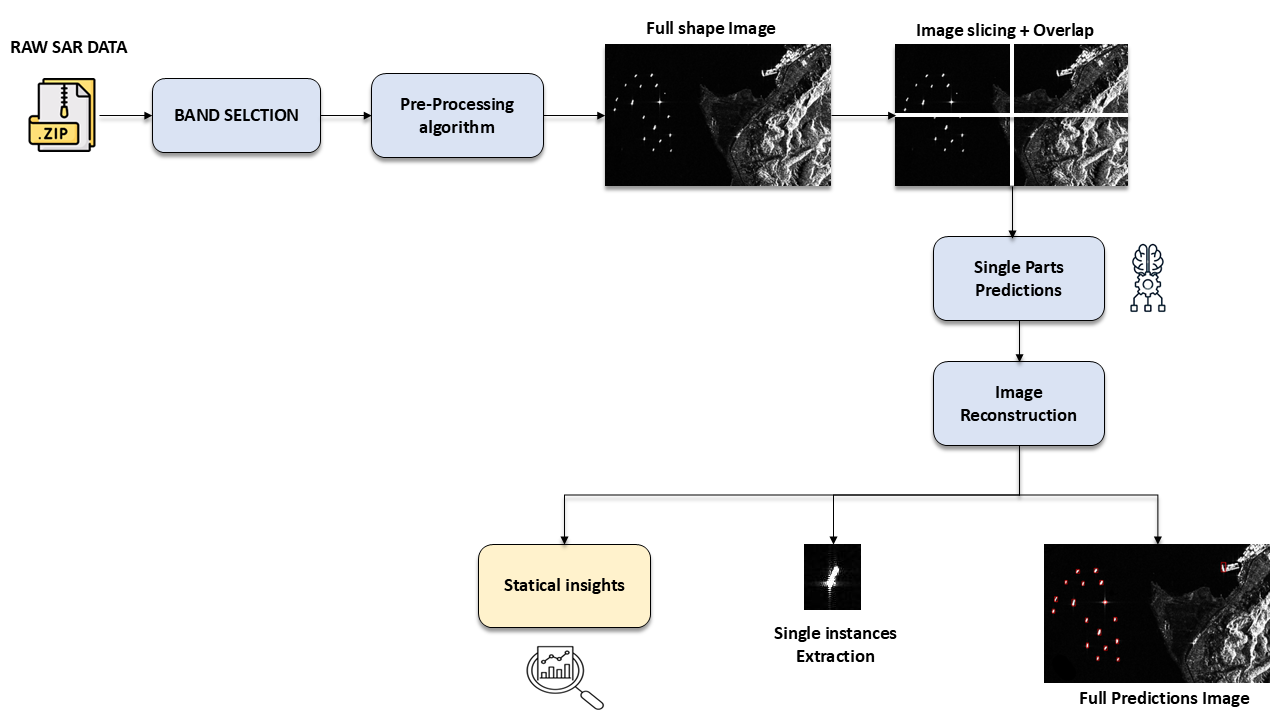
\includegraphics[width=1\linewidth]{apiprediction.png}
    \caption{RAW Data Prediction Algorithm Flowchart}
    \label{fig:raw_data_prediction_algorithm}
\end{figure}

\subsubsection{Google Earth Engine Prediction \acrshort{api}}
The proposed workflow delineates an advanced processing methodology for ship detection, leveraging user-defined geospatial inputs and data sourced from Google Earth Engine. The procedure initiates with the user specifying a region of interest (ROI) and a temporal range via an interactive map interface within the user interface (UI). Subsequently, relevant \acrshort{sar} data are downloaded from Google Earth Engine, tailored to the defined ROI and date range, facilitating precise data acquisition. This dataset undergoes preprocessing and model initialization to optimize its compatibility with the analytical framework.\\

The core analytical phase employs the inference slicer method, segmenting the preprocessed data into manageable subsets for detailed predictive modeling. This approach enhances computational efficiency and detection accuracy across the ROI. Outputs are rendered in an interactive UI, comprising statistical insights with quantitative metrics and graphical representations, isolated single-instance extractions for in-depth analysis, and a comprehensive full predictions image encapsulating the detection landscape.\\

This methodology ensures robust performance evaluation and operational efficacy, positioning it as a valuable tool for maritime surveillance and environmental monitoring applications. \begin{figure}[!ht]
    \centering
    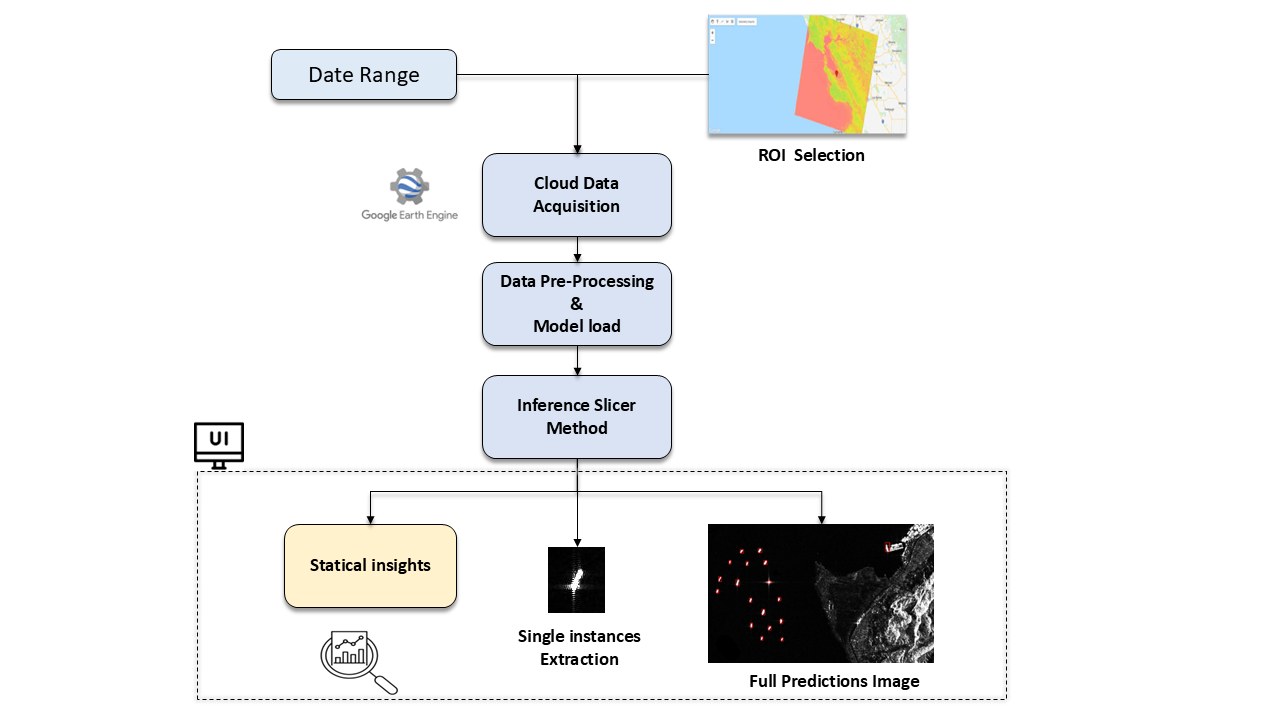
\includegraphics[width=1\linewidth]{engineAPI.png}
    \caption{Google Earth Engine Prediction \acrshort{api} Flowchart}
    \label{fig:gee_prediction_api}
\end{figure}

\subsection{Installation and Setup Guide}
\begin{itemize}
    \item Firstly, clone the repository \acrshort{sar}-SHIP-DETECTION. \item Download the dataset or use the link listed in the readme of the repository
    \item Download the model weights from the readme of the the repository
    \item Run:\begin{lstlisting}
pip install -r requirements.txt
\end{lstlisting}
\end{itemize}


For inference to the Jetson Nano use ssh to connect to the terminal. On windows a
program like PuTTY may have to be used, though ubuntu is recommended. An
alternative to directly writing onto the Jetson Nano is to secure copy (scp) the
project. Create a virtual python environment and install the required packages. The Jetson
Nano should already come equipped with \acrshort{tensorrt} among other packages with
the Jetson Nano \acrshort{sdk}. Format the model from \acrshort{onnx} format to \acrshort{tensorrt}, then
inference the model to the Jetson Nano. Finally, run the main python file. Make sure to specify the output location. \subsection{Configuation}
From the github repository, requirements.txt, the \acrshort{sar} dataset, and model \acrshort{onnx} file may
be necessary for setup. It is recommended that you follow section 6.1.3 and 6.1.4 to
install the necessary software and configure the hardware. \newpage
\section{Model Training and Optimization}
\subsection{Dataset Preparation Review}
After conducting preliminary research on public datasets containing Synthetic Aperture Radar (\acrshort{sar}) ship imagery, a shortlist of high-quality candidates was compiled. Upon closer evaluation, two datasets were selected: the \acrshort{sar} \acrshort{ssdd} Dataset and the \acrshort{sar} Ship Dataset. These datasets were merged to create a preliminary dataset, which was then used to train a minimum viable product (MVP) model.\\

Roboflow was used to upload and manage the datasets. Using the platform, the datasets were merged and split into training, validation, and test subsets. Roboflow also converted the data to the YOLOv11 format and resized the images to 640 by 640 pixels, the recommended input size for models in the YOLO family. No augmentation was applied to the preliminary dataset.

The final dataset builds upon the preliminary version by incorporating slightly lower-resolution public \acrshort{sar} data and edge cases such as vessels in glacial waters or near oil rigs. These additions enhance the model’s robustness and help reduce false positives.\\

The final dataset was annotated using Roboflow, with ship positions verified against Automatic Identification System (\acrshort{ais}) data corresponding to the \acrshort{sar} data acquisition period. Where available, optical imagery from similar timeframes was also used for verification. This validation process reduces the likelihood of human error during annotation, thereby minimizing the introduction of noise. Roboflow ensures high-precision bounding boxes, contributing to the overall quality of the annotated dataset.\\

The final dataset was then merged with the preliminary dataset using Roboflow. It was partitioned into training, validation, and test subsets in a 70\%, 20\%, and 10\% split, respectively.\\

To export the dataset for training in Google Colab or a similar environment, Roboflow provides three methods: direct download as a ZIP archive, cURL via the command-line interface, or use of the Roboflow Python package. \\

To install and access the dataset using the Roboflow package, the following commands can be used:
\begin{lstlisting}
!pip install roboflow
from roboflow import Roboflow

rf = Roboflow(api_key="API_KEY_HERE")
project = rf.workspace("WORKSPACE_NAME").project("PROJECT_NAME")
version = project.version(1)
dataset = version.download("EXPORT_FORMAT")
\end{lstlisting}
Roboflow also offers the option to automatically generate a Google Colab notebook pre-configured with the appropriate installation and dataset download commands. Users can initiate these commands by clicking the run button next to each code block. While Roboflow typically autofills dataset details, users should ensure that all required information is correctly specified. \subsection{Training Process}
The \acrshort{yolov11m} model for \acrshort{sar} ship detection was trained using a transfer learning strategy. We initialized the model with pre-trained weights from the \acrshort{coco}, allowing the network to adapt more efficiently to the \acrshort{sar} image domain. This approach significantly reduced training time and improved convergence stability.\\

Training was conducted on a Kaggle Notebook with access to a Tesla T4 GPU (16GB), running in a cloud-hosted environment with \acrshort{pytorch}, \acrshort{cuda} 11.x, and Python 3.10. This setup provided sufficient resources for training the medium-sized \acrshort{yolov11m} model on 640×640 \acrshort{sar} images.\\

Hyper-parameters used:
\begin{itemize}
    \item Model architecture: 231 layers
    \item Parameters: 20,053,779
    \item GFLOPs of computation: 68.2
    \item Learning rate: 0,002
    \item Momentum: 0.9
    \item Epochs: 20
    \item Image Size: 640×640 (for both training and validation)
\end{itemize}

Progress was tracked using TensorBoard and Ultralytics’ built-in training logger, reporting training/validation loss, precision, recall, \acrshort{map}@0.5, and \acrshort{map}@0.5:0.95. Visualizations of label distributions were saved automatically.\\

To train the \acrshort{yolov11m} model for \acrshort{sar} ship detection on Kaggle, follow these steps:
\begin{enumerate}
    \item Set Up the Kaggle Notebook Environment:
    \begin{itemize}
        \item Create a new Kaggle NotebookEnsure your Kaggle notebook has GPU enabled
        \item Install Ultralytics' YOLOv11 framework
        \begin{lstlisting}
        !pip install ultralytics --upgrade2
        \end{lstlisting}
    \end{itemize}

    \item Prepare the Dataset:
    \begin{itemize}
        \item Upload or mount your \acrshort{sar} ship detection dataset in YOLO format
        \begin{lstlisting}
        /images/train, /images/val, /labels/train, /labels/val
        \end{lstlisting}
        \item Create a dataset config \acrshort{yaml} file, e.g. \begin{lstlisting}
        data/sar_ship.\acrshort{yaml}:
        \end{lstlisting}
    \end{itemize}

    \item Run the Training Command
    \begin{lstlisting}
    !yolo detect train --model \acrshort{yolov11m}.\acrshort{yaml} --data data/sar_ship.\acrshort{yaml} \
    --epochs 20 --img 640 \
    --weights yolo11n.pt --device 0 \
    --project runs/train --name yolov11m_sar_ship \
    --workers 2
    \end{lstlisting}
\end{enumerate}

\subsection{Optimization techniques for Jetson Nano}
To ensure optimal performance in constrained environments characterized by low latency, embedded deployment, and strict power efficiency a rigorous optimization phase was conducted for the AI models. This process is structured into two key steps:

\paragraph{Conversion to \acrshort{onnx} (Open Neural Network Exchange)} Models initially trained in \acrshort{pytorch} are exported to the \acrshort{onnx} format, an interoperable standard that enables cross-framework optimization and deployment (e.g., \acrshort{tensorrt}, OpenVINO). This conversion leverages \acrshort{onnx}’s computational graph representation, which provides a unified intermediate format to encapsulate the model’s architecture, weights, and operations. By transitioning to \acrshort{onnx}, the process preserves model integrity while facilitating subsequent optimizations, allowing seamless portability across diverse hardware platforms and inference engines, thus enhancing scalability and deployment flexibility. \paragraph{Simplification of the \acrshort{onnx} Computational Graph} The exported \acrshort{onnx} graph undergoes structural simplification using tools like \acrshort{onnx}-simplifier or onnxruntime-tools. This involves:
\begin{itemize}
    \item \textbf{Removal of Redundant Layers}: Unnecessary operations such as Dropout, Identity, and Cast, which are typically employed during training but are redundant during inference, are systematically eliminated to reduce computational load. \item \textbf{Operator Fusion}: Compatible operations, such as Convolution followed by Batch Normalization and ReLU, are merged into a single optimized operation (e.g., FusedConv). This fusion reduces the number of sequential computations, minimizing memory accesses and improving execution speed.Mathematically, this ensures that ( $F_{\text{optimized}}(x) \approx F_{\text{original}}(x)$ ), where the approximation holds by maintaining the output distribution within an acceptable error margin (e.g., $<1\%$ deviation in mean squared error), while significantly reducing computational overhead and latency. This step is critical for embedded systems where resource constraints necessitate efficient graph traversal. \end{itemize}



\subsection{Model Deployment Pipeline}
This section outlines the end-to-end process for converting the trained \acrshort{yolov11m} model into an optimized inference format suitable for Jetson Nano deployment using \acrshort{tensorrt}. \begin{enumerate}
    \item \textbf{Export \acrshort{yolov11m} to \acrshort{onnx} Format}
    
    After training is complete, export the \acrshort{pytorch} .pt model to \acrshort{onnx} using Ultralytics’ built-in export command:
    \begin{lstlisting}
     !yolo export model=runs/train/yolov11m_sar_ship/weights/best.pt format=\acrshort{onnx}
     \end{lstlisting}
    \item \textbf{Transfer the \acrshort{onnx} Model to Jetson Nano}
    
    Copy the exported \acrshort{onnx} model to the Jetson Nano device using \acrshort{scp} or a USB drive:
    \begin{lstlisting}
    \acrshort{scp} runs/train/yolov11m_sar_ship/weights/best.\acrshort{onnx} jetson@<jetson_ip>:~/models/
    \end{lstlisting}
   
    
     
    \item \textbf{Convert \acrshort{onnx} to \acrshort{tensorrt} on Jetson Nano}
    
     On the Jetson Nano, use \acrshort{onnx}-\acrshort{tensorrt} or trtexec (included in NVIDIA JetPack) to convert the \acrshort{onnx} model to a \acrshort{tensorrt} engine:
    \begin{lstlisting}
    # Install \acrshort{onnx} and \acrshort{tensorrt} dependencies (if not already installed)
    sudo apt install python3-pip
    pip3 install \acrshort{onnx} onnxruntime
   
    # Convert to \acrshort{tensorrt} engine (\acrshort{fp16})
    trtexec --\acrshort{onnx}=best.\acrshort{onnx} --saveEngine=best_fp16.engine --\acrshort{fp16}
    \end{lstlisting}
 
   
 
    \item \textbf{Run Inference on Jetson Nano}
    
    Use a custom Python script or \acrshort{tensorrt}-compatible YOLO wrapper (like yolort or \acrshort{tensorrt}-yolov5) to perform inference. Example using \acrshort{onnx} Runtime:
    \begin{lstlisting}
     import onnxruntime as \acrshort{ort}
     import \acrshort{cv2}
     import \acrshort{numpy} as np
     
     session = ort.InferenceSession("best.\acrshort{onnx}")
     image = cv2.imread("test.jpg")
     input_tensor = preprocess(image)  # Resize, normalize, etc.
     
     outputs = session.run(None, {session.get_inputs()[0].name: input_tensor})
     postprocess(outputs)
    \end{lstlisting} 
\end{enumerate}


\begin{figure}[!ht]
    \centering
    
\includegraphics[width=0.35\linewidth]{flow_depl.png}
    \caption{Model Deployment Pipeline Diagram }
    \label{fig:model_deployment_pipeline}
\end{figure}

\newpage


\section{Evaluation and Testing}
\subsection{Test Plan And Methodology}
Test Plan and Methodology
Testing is a critical phase in AI model development, as it evaluates the model's performance and identifies areas requiring refinement. The testing methodology for ship detection in SAR (Synthetic Aperture Radar) images involves multiple approaches to ensure robustness and accuracy. \begin{itemize}
    \item \textbf{Single-Image and Batch Testing}
    
    The model is evaluated on individual images or curated test sets to analyze detection performance. Misclassifications such as false positives (e.g., oil rigs mistaken for ships) or false negatives are examined to determine weaknesses. These insights guide further preprocessing adjustments or targeted retraining on problematic cases. \item \textbf{Performance Metrics and Learning Curves}
    
    During training, validation metrics such as mean Average Precision at IoU 50 (mAP@50), Precision, and Recall are tracked. These metrics are visualized in learning curves to assess the progress and convergence of the model. A divergence between training and validation performance may indicate overfitting, prompting adjustments in hyperparameters or dataset composition. \item \textbf{Iterative Refinement Based on Test Results}
    
    If the model exhibits specific failure modes (e.g., confusion between ships and offshore structures), targeted datasets are introduced to improve discrimination. For instance, if oil rigs are frequently misclassified, supplemental training data containing rigs is incorporated to enhance feature learning. This iterative process ensures continuous improvement in detection accuracy.
\end{itemize}

By systematically applying these methods, the model’s reliability in real-world SAR ship detection scenarios is rigorously validated. \subsection{Performance Metrics}
To evaluate the performance of the ship detection model on SAR images, the following metrics are employed:
\subsubsection{Detection Accuracy Metrics}
\begin{itemize}
    \item \textbf{False Positives} (FP): Instances where the model incorrectly identifies a non-ship object (e.g., oil rigs, waves) as a ship. \item \textbf{False Negatives} (FN): Instances where the model fails to detect actual ships. \item \textbf{Mean Average Precision} (mAP@IoU):
    
    The primary metric for object detection, mAP@0.50 calculates the mean precision across all recall levels at an Intersection over Union (IoU) threshold of 0.50. A higher IoU threshold (e.g., mAP@0.75) enforces stricter localization accuracy. $$IoU=\frac{\text{Area of Overlap}}{\text{Area of Union}}$$
    \item \textbf{Precision}: Measures the proportion of correct ship detections among all predicted ships: $$\text{Precision} = \frac{\text{True Positives (TP)}}{\text{TP + False Positives (FP)}}$$
    
    \item \textbf{Recall}: Measures the proportion of actual ships correctly detected:$$\text{Recall} = \frac{\text{TP}}{\text{TP + False Negatives (FN)}}$$
    
    \item \textbf{F1-Score}: The harmonic mean of precision and recall, balancing both metrics:
    $$F1 = 2 \times \frac{\text{Precision} \times \text{Recall}}{\text{Precision} + \text{Recall}}$$
\end{itemize}
 
These metrics collectively quantify the model’s detection accuracy and guide refinements (e.g., addressing false alarms from offshore structures).

\subsubsection{Inference Efficiency Metrics}
\begin{itemize}
    \item \textbf{Latency}: Time taken to process a single SAR image during inference. Lower latency is critical for real-time applications.

    \item \textbf{Memory Usage}: GPU/RAM consumption during inference, particularly relevant for edge deployment. \item \textbf{Power Consumption}: Energy efficiency, measured in watts, for deployment on resource-constrained devices (e.g., drones, satellites). \end{itemize}

\subsection{Experimental Setup}
\paragraph{Model Selection}
For our ship detection project, we implemented Ultralytics' YOLOv11m model. As demonstrated in comparative benchmarks (Figure X), YOLOv11 offers an optimal balance between detection accuracy and processing speed - a critical requirement for SAR-based maritime surveillance. The medium-sized "m" variant was selected to maintain reasonable computational efficiency while preserving detection performance, particularly for small vessels in complex SAR imagery. \paragraph{Hardware Configuration}
The training platform consisted of:

\begin{itemize}
    \item \textbf{Development System:} Windows 11 workstation with NVIDIA RTX 3090 GPU (24GB VRAM)
    \item \textbf{Deployment Target:} NVIDIA Jetson Nano GPU (128-core Maxwell, 4GB RAM) to simulate edge-computing constraints
\end{itemize}


\paragraph{Core Framework}
\begin{itemize}
    \item \textbf{\acrshort{pytorch} 2.0:} Selected for its dynamic computation graph and robust ecosystem for computer vision tasks
    \item \textbf{Ultralytics YOLOv11 implementation:} Provides optimized architectures and training pipelines
\end{itemize}

\paragraph{Training Infrastructure}
\textbf{Roboflow SaaS platform:} Enabled cloud-based dataset management and training with the following capabilities:
\begin{itemize}
    \item Dataset versioning and preprocessing (augmentations, resizing)
    \item Distributed training on cloud GPUs during inactive local hours
    \item Free tier limitations: 100 training credits/month (equivalent to $\sim$1,000 annotated images)
\end{itemize}

\paragraph{Additional Tools}
\begin{itemize}
    \item \textbf{LabelImg:} Used for manual annotation refinement
    \item \textbf{OpenCV:} Applied for SAR-specific preprocessing
    \item \textbf{TensorBoard:} Utilized for training monitoring
\end{itemize}

\paragraph{Dataset Considerations}
To address Roboflow's credit constraints:
\begin{itemize}
    \item Implemented aggressive image tiling to maximize usable samples
    \item Prioritized diversity in ship types and sea conditions
    \item Used offline augmentation for credit-free dataset expansion
\end{itemize}

\paragraph{Datasets}

We employed a combination of public and augmented datasets to ensure robust model generalization:

\begin{table}[h!]
\centering
\begin{tabular}{|l|l|l|}
\hline
\textbf{Dataset} & \textbf{Source} & \textbf{Characteristics} \\
\hline
SAR Ship Dataset & OPENSAR Project & High-resolution SAR imagery \\
SSDD Dataset     & GitHub/Official-SSDD & Annotated ship detections \\
\hline
\end{tabular}
\caption{Summary of Datasets Used}
\end{table}

\paragraph{Data Processing}

\begin{itemize}
    \item \textbf{Annotation:} Custom labeling was performed using CVAT to address specific challenges (e.g., oil rig/ship discrimination) not fully covered by public datasets. \item \textbf{Augmentation:} Applied transformations such as rotation, noise injection, and contrast adjustment to enhance dataset variability without collecting new imagery. This proved particularly valuable for improving model resilience to SAR-specific artifacts. \end{itemize}

\paragraph{Training Protocol}

The model was initially trained on local hardware using \acrshort{pytorch}, with periodic validation on Roboflow to monitor progress. Final tuning incorporated:

\begin{itemize}
    \item Transfer learning from COCO pretrained weights
    \item Progressive resizing to adapt to SAR image dimensions
    \item Focused retraining on challenging cases (e.g., clustered ships)
\end{itemize}


%\subsection{Results and Analysis}
%TODO

%\subsection{Validation and Verification Against Requirements}
%TODO

%\subsection{Deployments \& Optimization}

\newpage
\section{Future Work and Enhancements}
Future advancements in this project aim to significantly enhance the robustness, scalability, and practical applicability of the synthetic aperture radar (\acrshort{sar})-based ship detection and tracking system, addressing current limitations and expanding its operational scope.\\

In the realm of advanced algorithms, the exploration of cutting-edge techniques such as transformer-based detectors will be prioritized to elevate detection precision by leveraging self-attention mechanisms that excel in capturing long-range dependencies within \acrshort{sar} imagery, surpassing the capabilities of conventional convolutional neural networks. Additionally, multi-sensor data fusion will be pursued to synergistically combine \acrshort{sar} data with real-time Automatic Identification System (\acrshort{ais}) feeds, enabling more accurate tracking of vessels, while predictive modeling will be developed to forecast the trajectories of lost ships and detect oil spills through anomaly detection algorithms tailored to \acrshort{sar} signatures. \\

For real-time deployment, the focus will shift toward optimizing system performance under operational constraints, including minimizing latency through efficient edge computing pipelines and managing continuous data streams from dynamic maritime environments. A key strategy involves deploying the system on Nano-satellite platforms in orbit, which will necessitate the design of lightweight inference models compatible with constrained computational resources, ensuring persistent global coverage and real-time monitoring capabilities. \\

The dataset will be substantially expanded to incorporate a broader spectrum of \acrshort{sar} data, including diverse polarizations (e.g., \acrshort{vv} and \acrshort{vh}) to enhance metallic surface detection, varying resolutions to address different operational ranges, and data from extreme environmental conditions such as icebergs and oil rigs, thereby improving model generalization and resilience across heterogeneous maritime scenarios. Integration with other systems will involve interfacing the developed framework with existing maritime surveillance platforms to enable seamless data exchange, connecting with command and control systems for tactical decision-making, and leveraging cloud services like Streamlit to facilitate scalable data processing, storage, and interactive visualization for stakeholders.\\

Furthermore, user interface development will focus on crafting a highly interactive and intuitive interface, incorporating advanced visualization tools such as 3D geospatial mapping and real-time anomaly heatmaps, to empower users with enhanced interaction capabilities and expedite operational decision-making processes based on the system’s outputs. \newpage
\section{Conclusion}
The \acrshort{sar} Ship Detection Project represents a significant advancement in maritime surveillance by leveraging Synthetic Aperture Radar (\acrshort{sar}) imagery and state-of-the-art machine learning techniques. Through the integration of robust preprocessing pipelines, optimized \acrshort{yolov11m} models, and edge-computing deployment on the NVIDIA Jetson Nano, the project successfully addresses critical challenges such as speckle noise, varying ship sizes, and cluttered environments. The system's three-tiered accessibility spanning edge devices, web-based interfaces, and direct image uploads ensures versatility for diverse operational scenarios, from illegal fishing monitoring to search and rescue missions.\\

Key achievements include the development of a high-accuracy detection framework with a mean average precision (\acrshort{map}) exceeding 90\%, real-time processing capabilities, and seamless integration with \acrshort{ais} data for enhanced tracking reliability. The iterative preprocessing workflow, featuring advanced techniques like polarimetric band selection, adaptive thresholding, and land masking, significantly reduces false positives while preserving target integrity. Furthermore, the project's modular design and comprehensive documentation facilitate future scalability and adaptation to emerging technologies, such as transformer-based detectors or multi-sensor fusion.\\

Looking ahead, the system's potential for deployment on CubeSats and integration with global maritime networks promises to revolutionize real-time, all-weather maritime domain awareness. By bridging the gap between \acrshort{sar} data availability and actionable intelligence, this project lays a foundation for safer, more secure, and sustainably managed oceans. Future work will focus on expanding datasets, refining edge-optimized models, and enhancing user interfaces to further solidify the system's role in modern maritime operations.\\

In summary, the \acrshort{sar} Ship Detection Project not only meets its immediate technical and operational goals but also paves the way for innovative applications in environmental monitoring, defense, and global trade, underscoring the transformative power of AI-driven \acrshort{sar} analytics. \newpage

\printglossaries
\newpage
\printbibliography


\end{document}